\documentclass[pdftex,12pt,a4paper]{report}

% Some useful packages.
\usepackage{amsmath}
\usepackage{siunitx}
\usepackage{graphicx}
\usepackage{verbatim}
\usepackage{mhchem}
\usepackage{textcomp}
\usepackage{setspace}

% Reduces margins substantially.
\usepackage{geometry}
\newgeometry{margin=2.5cm}

% Allows headers and footers.
\usepackage{fancyhdr}
\pagestyle{fancy}
% Get rid of annoying line under header.
\renewcommand{\headrulewidth}{0pt}

\lhead{}
\chead{}
\rhead{}

% Turn on subsubsection numbering.
% \setcounter{secnumdepth}{3}

\newcommand{\ts}{\textsuperscript}
\newcommand{\HRule}{\rule{\linewidth}{0.5mm}}

% Harvard style references.
\usepackage[backend=biber,style=authoryear,sorting=nyt,dashed=false]{biblatex}
\renewcommand*{\nameyeardelim}{\addcomma\space}
\addbibresource{references/references.bib} % note the .bib is required

% 12,000 words max.

% overall structure:
% Abstract
% Intro
% Data Sources
% Development of the Hurricane Detection Procedure
% Conclusion
% Appendices
% References

% Common typos:
% possibly

% TODOs: 4

\title{Objective Tracking and Classification of Hurricanes in the 20\ts{th} Century Reanalysis Dataset}
\author{Mark Muetzelfeldt - UCL Department of Geography}

\date{29 August, 2014}

\begin{document}

\begin{titlepage}

\begin{center}

\textsc{\LARGE University College London}\\[1.5cm]

\textsc{\Large MSc Environmental Modelling Dissertation}\\[0.5cm]

% Title
\HRule \\[0.4cm]
{ \LARGE \bfseries Objective Tracking and Classification of Hurricanes in the 20\ts{th} Century Reanalysis Dataset \\[0.4cm] }

\HRule \\[1.5cm]

% Author and supervisor
\begin{minipage}{0.4\textwidth}
\begin{flushleft} \large
\emph{Author:}\\
Mark \textsc{Muetzelfeldt}
\end{flushleft}
\end{minipage}
\begin{minipage}{0.4\textwidth}
\begin{flushright} \large
\emph{Supervisors:} \\
Dr.~Chris \textsc{Brierley} \\
Qinling \textsc{Wu}
\end{flushright}
\end{minipage}
\\[0.5cm]
29\ts{th} August, 2014
\\[0.5cm]

This research dissertation is submitted for the MSc Environmental Modelling at University College London


\vfill
% Bottom of the page

\end{center}

\end{titlepage}


% Magic incantation to make a blank page with no page number that does not mess up page ordering.
\clearpage
\thispagestyle{empty}
\null
\addtocounter{page}{-1}%
\newpage

\onehalfspacing
\section*{Abstract}

% Should be <= 400 words.
% Not included in word count.
% ~369 words so far.
A procedure for the detection of hurricanes in the 20\ts{th} Century Reanalysis Project dataset is
developed. Tracks are derived from the dataset by tracking vorticity maxima over time. These derived
tracks are matched against best tracks taken from the International Best Track Archive for Climate
Stewardship (IBTrACS) best tracks dataset. Six different tracking configurations are evaluated:
using the vorticity at 0.995 times the surface and \SI{850}{hPa} pressure levels and using the
original resolution data, data downscaled by cubic interpolation to two and three times the original
resolution. It is found that using downscaling to three times the resolution provides a better match
between the derived tracks and the best tracks. Tracks at the different pressure levels produce
similar results, and the \SI{850}{hPa} pressure level is chosen on theoretical grounds.

The derived tracks are used to obtain extra fields from the 20\ts{th} Century Reanalysis
Project dataset, such as the local minimum pressure and the temperature at the \SI{850}{hPa}
pressure level. These extra fields, along with the information obtained by matching the derived
tracks to the best tracks, are used to produce training and validation datasets for supervised
machine learning classification algorithms. Different classification algorithms are evaluated based
on classification success and error metrics. It is found that a Stochastic Gradient Descent
classifier performs best based on these metrics.

The hurricane detection procedure is run over the course of the 20\ts{th} century, and a comparison
between the estimated number of hurricanes and the number as recorded in the IBTrACS dataset is
performed. It is found that there is good correlation between the two time series, and that there
are significant discrepancies between the two series between 1890 to 1914 and 1945 to 1965. Between
1890 and 1914, the estimated hurricane count is higher than the best tracks count. Between 1945 and
1965, fewer estimated hurricanes are found than best tracks hurricanes. 

A downwards trend in both the estimated and best tracks hurricanes is detected from 1890 to 1914. An
upwards trend in the number of hurricanes from 1966 to 2009 is also detected from the estimated
number of hurricanes, although this may be due to detecting fewer hurricanes in the 1960s and 1970s.

\begin{center}
\textbf{Word count:} 11925 % 28/08/14 10:48
\end{center}

\newpage
\section*{Acknowledgements}

I would like to thank Dr. Chris Brierley for his guidance and assistance in this dissertation.
Technical expertise from Qinling Wu proved useful in setting the direction for this project.
Talking to Joshua Studholme helped to provide context for the field and ideas for analysis, as well
as giving me some pointers on extratropical transitions.
Dr. Kevin Hodges (Reading University) provided many useful suggestions for the tracking algorithm.
NERSC and the National Climatic Data Center at the NOAA both provided excellent resources in the
20\ts{th} Century Reanalysis Project and the IBTrACS projects, with the first of these providing
over 1.3 terabytes of data.
Finally, numerous discussions with Robert Muetzelfeldt were invaluable for keeping me on track and
for sounding out various ideas.

\newpage

\tableofcontents

% Everything from here to auto-critique is included in word count.
\chapter{Introduction}
% From the dissertation handbook:
% Introduction, presenting the research problem, rationale, context and outline objectives,
% aims/objectives (possibly as a formal hypothesis).

% Rationale.
% ----------

% Impacts of hurricanes.
Hurricanes are one of nature's most impressive and devastating extreme weather events. The costliest
hurricane this century, hurricane Katrina, was responsible for 1833 deaths and caused \$108
billion USD in damage \parencite{knabb2006tropical}.
Hurricanes are therefore of great importance socially,
economically and, in hurricane Katrina's case, even politically \parencite{kellner2007katrina}.

% Heat transport by hurricanes.
Hurricanes, and more generally tropical cyclones, are also known to be a major contributor to the
poleward heat flux that evens out the temperatures between the poles and the tropics, carrying an
estimated \SI{1.4e15}{W} towards the poles \parencite{emanuelContribution2001}. This
contribution is large enough that it may affect the thermohaline circulation
\parencite{hu2009effect}, a major component of the coupled atmosphere-ocean system of the Earth. So,
coupled with their socio-economic impact, understanding hurricanes is of intrinsic scientific
interest too, helping to understand the Earth's climate and to produce more accurate General
Circulation Models (GCMs).

% Effects of global warming on frequency/intensity.
From a theoretical perspective, increasing global mean temperatures are predicted to lead to an
increase in the intensity of hurricanes \parencite{emanuel1987dependence}. This is backed up by
computer modelling, which predicts an average of 6\% increase in maximum wind speed under conditions
of a rise in global temperatures of \SI{0.8}{\textdegree C} to \SI{2.4}{\textdegree C} over the next
80 years \parencite{knutson2004impact}. Given that a hurricane's destructive potential varies as the
maximum surface wind speed cubed \parencite{emanuel2005increasing}, this would lead to a 20\%
increase in hurricanes' destructive potential. In line with the theory, this destructive potential
is found to have risen ``markedly'' since the 1970s \parencite{emanuel2005increasing}. As well as
increases in the intensity of hurricanes, increases in their frequency have been detected
\parencite{goldenberg2001recent, holland2007heightened}.

% Trends in hurricanes over time leading on to...
Most studies into hurricane frequency and intensity tend to rely on best tracks databases as their
primary data source, such as the IBTrACS database used in this study
\parencite{knappInternational2010}, or the tropical cyclone database from the National Hurricane
Center \parencite[HURDAT;][]{jarvinen1984tropical}. These databases collect information from a
variety of different sources: land-based stations, ships, aircraft reconnaissance and satellite
images. Due to some of these sources not being available over the course of the 20\ts{th} century,
these databases suffer from some problems when going into the middle and early 20\ts{th} century,
such as the lack of satellite data before the 1970s, and the lack of reliable aircraft
reconnaissance data before the mid 1940s \parencite{chang2007number}. 

Accordingly, in this study, the approach taken is a different one. Instead of using the numbers
compiled by various agencies as the primary source of information on hurricanes, the primary data
will be taken from global reanalysis data, specifically the 20\ts{th} Century Reanalysis (20CR)
Project \parencite{compoTwentieth2011}. Hurricanes will be detected in these data, and the detection
procedure will be trained and validated on recent data (from 1990 to 2009), where reliable best
tracks exist. Once the detection procedure has been trained, it can be used to run over the entire
20\ts{th} century, providing an objective measure of the number of hurricanes in each year. This
will allow for an estimation of the hurricane frequency that is not solely based on the best tracks
records, and therefore less susceptible to the changes in these best track records over time. This
estimation will be almost independent of the best tracks records, although given the 20CR project
assimilates information from IBTrACS it cannot be said to be totally independent (see Section
\ref{sec:ispd}).

% \section{Research Problem}
% Detection of hurricanes in 20CR dataset.
% * Reason: spans 20th C.
% * List other reanalyses that do not.
% * Problems with this dataset: low resolution, despite trying to make it objective, it will likely
% change over time, making trend detection tricky (laying groundwork for talking about this in
% discussion).

% Mention NCEP/NCAR Reanalysis 1
% Mention ERA-40
% Mention JRA-55

% BRIEF description of what reanalysis is,
% A global reanalysis project is an attempt to reconstruct the complete historical state of the
% atmosphere at a given spatial and temporal resolution, assimilating an incomplete series of
% measurements of atmospheric variables (a more complete description is given in Section
% \ref{sec:20crp}). 
% Several reanalysis projects exist, such as NCEP/NCAR Reanalysis \parencite{kalnay1996ncep,
% kistler2001ncep}, ECMWF ERA-40 \parencite{uppala2005era} and the JRA-55
% \parencite{ebita2011japanese}. These reanalysis only go back to 1948, 1957 and 1958  respectively,
% and so would not be useful for looking into hurricanes at the start of the 20\ts{th} century. The
% 20CR on the other hand covers over 140 years, from 1871 to 2012, and is therefore suitable for
% studying the number of hurricanes across the entire 20\ts{th} century. It contains an estimate of
% the state of the atmosphere on a T62 (2\textdegree) spatial resolution and at 6-hourly timesteps,
% with variables such as the longitudinal and latitudinal wind speeds at the 0.995 times the surface
% pressure level, or the Near Surface Pressure Level (NSPL), and the temperature at the \SI{850}{hPa}
% pressure level recorded.

\section{Existing Tracking and Detection Algorithms}
% Context.
% --------

% Tracking/detection: Literature review. Lots and lots of references.
% Tracking: why it's a good idea to track then detect. Links to Hodges 1 and 2.
% Detection: GCM:
% Talk about role of resolution
% Talk about
% Discuss different approaches.
% Detection: Reanalyses.
% List some previous attempts to detect hurr/tropical cyclones in reanalyses.
% Talk about the primary difference: the existence of best tracks datasets.

Numerous studies have looked into the detection of hurricanes, both in the output of GCMs and in
global reanalysis datasets. Several reasons exist for wanting to detect hurricanes in the output of
GCMs. Often the goal is to look into the effects of climate change with a warming climate
\parencite{bengtsson1996will, sugi2002influence}. When running this sort of
analysis, there is no objective measure of whether or not an individual detection of a hurricane is
correct or not, although often tests are done to make sure that the resulting climatologies are
realistic. This is in contrast to running the detection using a
reanalysis dataset, where it is possible to match the detected hurricane to a given
tracks in a given best track database, as was done in \textcite{walsh1997objective}. Detection of
hurricanes can also be used to compare the climatologies in different reanalysis projects, as was
done in \textcite{trigo2006climatology}. The detection of hurricanes in climatological datasets
taken either from reanalysis datasets and output from GCMs is otherwise technically similar.

There are two closely related approaches to detecting hurricanes in climatological datasets. The
first is to examine the dataset at every timestep, looking for a cell or cells which meet certain
criteria, and then produce tracks based on combining cells that meet these criteria in different
timesteps. These criteria normally involve vorticity at the \SI{850}{hPa} pressure level,
maximum wind speed, and temperature anomalies at different pressure levels. Additionally, the tracks
produced have to be longer than a certain time duration, typically 1.5 to 2 days. Examples of
studies that take this approach are \textcite{bengtsson1995hurricane, walsh1997objective}.

The second approach of detecting hurricanes is to first track some feature from one timestep to the
next (typically vorticity maxima), and then apply a set of criteria to each point in these tracks to
see whether they represent hurricanes or not. Normally, a time duration of the tracks must be longer
than a certain duration as well, again typically 1.5 days. These tracks can yield extra information
about the hurricanes, such as where they were formed, which is important in deriving details about
cyclogenesis \parencite{marchok2002ncep}. Useful information about the fate of the cyclone can also
be found, such as whether it undergoes an extratropical transition
\parencite{studholme2014objective}. This is the approach taken by \textcite{thorncroft2001african,
camargo2002improving}, and is also the approach that will be used in this study.

Both these approaches rely on thresholds being set for the criteria in advance of running the
detection procedure, although there may be some sensitivity analysis done on these thresholds as in
\textcite{walsh1997objective}. These thresholds can be somewhat arbitrary and can vary with resolution
\parencite{walsh2007objectively}. Two studies that have looked at T63 resolution (very close to the T62 used by
the 20CR dataset), have used values of \SI{6e-5}{s^{-1}} as a threshold value for hurricanes in the
\SI{850}{hPa} vorticity \parencite{bengtsson2006storm, bengtsson2007may}. Therefore any value for
this vorticity threshold used in this study should be of a similar magnitude to this number. The
thresholds can also vary from basin to basin \parencite{camargo2002improving}, and thus need to be
chosen quite carefully.

This study takes a different approach to choosing these thresholds. Instead of deciding what they
should be before running the analysis, the analysis is run, and the values of e.g. vorticity and
temperature at the \SI{850}{hPa} pressure level are recorded for each point along each track. Due to
the matching of the tracks derived from the 20CR data and the best tracks, it is then possible to
see which values of these fields correspond to hurricanes, and which do not. This allows for setting
of the thresholds \textit{after} the bulk of the processing has been done, thus greatly speeding up
the process of finding optimum values for these thresholds. It also permits the use of machine
learning classification algorithms, which it is hoped will improve the accuracy of the hurricane
detection, as measured by the number of true and false positives. Investigating the effect of
changing these thresholds is a similar approach to \textcite{walsh1997objective}, who analysed the
numbers of false and missing tropical cyclones over September 1989 and October 1992, and
investigated the changes in these number due to changing e.g. the vorticity threshold. The results
of this study will be compared against the results of \textcite{walsh1997objective} in Section
\ref{sec:classification_success}. 

% It bears repeating that this approach is only possible because
% this study is running the hurricane detection over a historical reanalysis dataset, otherwise this
% would not be possible, as there is no objective standard by which to judge success.

\section{Goals and Objectives}
% Objectives/Project Structure.
% -----------------------------
% Outline of objectives for this project.
% Finish with a run-down of the structure of the rest of the dissertation, including why it deviates
% from the traditional Intro/Methods/Results/Discussion/Conclusion structure.

The two principal goals of this study are to produce a hurricane detection procedure that is capable
of detecting hurricanes in the 20CR dataset, and to use this procedure to investigate hurricane
frequencies over the course of the 20\ts{th} century. These goals will be met by completing the
following objectives:

\begin{itemize}
    \item Develop a tracking algorithm that is capable of producing tracks derived from the 20CR
    \item Match the derived tracks to the tracks in the IBTrACS best tracks database
    \item Compare different tracking algorithm configuration, and choose the optimum tracking
        algorithm based on the overall distance between the tracks it produces and the best tracks.
    \item Collect extra information for each of the points in the optimum tracks, such as
        temperature at \SI{850}{hPa}
    \item Train different classification algorithms to correctly predict whether each point is a
        hurricane or not, by using the extra information, along with the information about whether a
        particular point is matched to a hurricane
    \item Choose the classification algorithm which performs best on success and error metrics, and
        this process will form the hurricane detection procedure
    \item Run this procedure over the course of the 20\ts{th} century
    \item Calculate aggregate statistics about the number of hurricanes over this duration
    \item perform a comparison between the estimated number of hurricanes from the 20CR dataset and
        the IBTrACS database
\end{itemize}

% Old form:
% The objectives of this study are to develop a tracking algorithm that is capable of producing tracks
% derived from the 20CR dataset that can be successfully matched to the tracks in the IBTrACS best
% tracks database. Following from this, these derived tracks will be used to collect extra information for
% each of the points in the track, such as temperature at \SI{850}{hPa}. This information will then
% used, along with the information about whether a particular point corresponds with a hurricane or
% not, to train different classification algorithms to correctly predict whether each point is a
% hurricane or not. The classification algorithm which performs best on success and error metrics will
% be chosen, and this process will form the hurricane detection procedure. This will then be run
% over the course of the 20\ts{th} century, and aggregate statistics about the number of hurricanes
% over this duration will be presented, along with a comparison between the estimated number of
% hurricanes from the 20CR dataset and the IBTrACS database.

The following chapter will present more detail on the two data sources used in this study: the 20CR
dataset and the IBTrACS database. Chapter \ref{chap:hurricane_detection_proc} will then detail the
steps in the hurricane detection procedure, presenting a logical progression of the procedure along
with results pertinent to the following sections in that chapter. Chapter
\ref{chap:results_analysis} will then look into the results of running the procedure over the course
of the 20\ts{th} century.  Chapter \ref{chap:discussion} will then discuss these results in the
wider context of hurricane detection and trends over the 20\ts{th} century, and Chapter
\ref{chap:conclusion} will provide a conclusion of the findings. This deviates slightly
from the traditional dissertation structure due to the desire to present the hurricane detection
procedure in a logical manner where the subsequent sections depend on the results of the previous
sections.

\chapter{Data Sources}

\section{20\ts{th} Century Reanalysis Project}
\label{sec:20crp}
% Key points:
% * Global reanalysis 1871-2012
% * Uses only SST, surf press, sea ice
% * Relatively bias free because of above (compared to say ERA-40)
% * spatio-temporal resolution
% * includes uncertainty
% * 56 ensemble members
The 20\ts{th} Century Reanalysis Project (20CR) is a project whose aim is to produce a consistent
best estimate of the state of the atmosphere by including information from a variety of different
sources \parencite{compoTwentieth2011}. Sea Surface Temperature (SST) and
sea ice data from the Hadley Centre Sea Ice and SST dataset \parencite{rayner2003global} are used to drive
a GCM - the NCEP Global Forecast System \parencite{kanamitsu1989description}.
This is combined with pressure observations from the International Surface Pressure Databank
\parencite{yin2008international}, which are assimilated with the forecasts provided by the GCM by
means of an Ensemble Kalman Filter (EKF). It provides estimates at a 2\textdegree\ spatial
resolution, and on a 6-hour timestep, from 1871 to 2012 (more years will be added in due time). A
level of consistency is ensured by using the same process from the beginning of the reanalysis to
the end, and by using only SST, sea ice and pressure data. This avoids the problems seen in other
reanalysis projects, such as ERA-40 \parencite{uppala2005era}, which incorporate as much data as
possible. This biases more recent years, as e.g. satellite data from the 1970s onwards provides far
more observations than exist before this period. 

% CULLED
% Due to the use of an EKF, it is also possible for
% the 20CR to provide estimates for the uncertainty of each of its estimates at each timestep,
% although this information is not used as part of this study.

% necessity of analysing single EM (ref compo2011)
The GCM and EKF are run with 56 ensemble members, meaning that for every timestep there are 56
estimates for the state of the atmosphere. An individual ensemble member consists of a GCM instance.
According to \textcite{compoTwentieth2011}, individual tracking of storms is best done through
tracking them in individual ensemble members, instead of looking at the ensemble mean. This is
because the ensemble mean, in the presence of only a few observations, exhibits less synoptic
variability. This is to say that in the absence of observations, each GCM instance acts almost
independently of the others. Thus when the mean of the ensemble members is taken, an atmospheric
feature that is present in all of GCM instances, but in slightly different locations, may not be as
evident. Therefore it is important that the individual ensemble members are used for detection of
atmospheric features such as hurricanes, and that is what is done in this study. Consequently, the
analysis carried out in this study had to be repeated 56 times, and this provides the classification
algorithms used in Section \ref{sec:classification} far more samples than if the ensemble mean or
only one ensemble member had been used. 

% CULLED
% , whose output will be updated in the presence of pressure observations as detailed in Section
% \ref{sec:technical_details}
% It also allows for the use of aggregate statistics from all
% of the ensemble members to be generated, such as the spread shown in Figure
% \ref{fig:20th_century_hurricane_timesteps}.

\subsection{Technical Details}
\label{sec:technical_details}
% How it works:

% Runs a GCM - NCEP GFS - to produce background fields
% Technical details on GCM
\subsubsection{GCM}
The GCM used for the reanalysis was the NCEP Global Forecast System
\parencite{kanamitsu1989description}, with
parameterisation as specified by \textcite{saha2006ncep}. The version used in the reanalysis was
slightly modified to permit time varying \ce{CO2} and volcanic aerosols. These, along with incoming
radiation, were used as specified in \textcite{saha2010ncep}. The model was run at a horizontal
resolution of T62 and a vertical resolution of 28 vertical hybrid sigma-pressure levels as described
by \textcite{juang2005discrete}. 

% CULLED
% This horizontal resolution is between the T42 and T106 resolutions
% analysed in \textcite{bengtsson1995hurricane}, and therefore should be capable of producing
% hurricane-type vortices, as the T42 model in that study was found to be capable of producing
% vortices, although it was noted that these vortices were of lower intensity and that their overall
% structure was less realistic than in the T106 GCM.

\subsubsection{EKF}
% Technical details EKF
The EKF is similar to the Monte Carlo approximation proposed by \textcite{evensen1994sequential,
evensen2003ensemble}. It is `deterministic', and is based on the `Ensemble Square Root Filter' of
\textcite{whitaker2002ensemble}. It works by taking the state of the atmosphere from the
56 instances of the GCM - which is the prediction by the model in Kalman filter terminology - and
updating this prediction based on the pressure observations at that timestep. Each individual
ensemble member is updated in such a way so as to keep the state of its atmosphere continuous,
whilst still incorporating the pressure observations (with one slight caveat; see the last paragraph
in the next section for details). To mitigate the effects of ``filter divergence'', whereby the
state of the EKF becomes too dependent on the output of the model, and does not give enough weight
to the observations, two methods are used. The first is to use covariance inflation, as described in
\textcite{whitaker2004reanalysis}. The second is to use covariance localisation, as described in
\textcite{houtekamer2001sequential}. 

% CULLED
% These are mentioned for completeness; a more detailed
% description is given in \textcite{compoTwentieth2011}.

% Assimilates the observations and the output from the GCM using an EKF to provide an estimate as to
% the state of the atmosphere at each timestep

\subsubsection{Production Process}
The process by which estimates are produced involves three main steps:

\begin{enumerate}
    \item Spin up of GCM
    \item Assimilate pressure data using the EKF
    \item Use GCM to predict the state of the atmosphere at the next timestep (go to step two)
\end{enumerate}

% CULLABLE
56 individual instances of the GCM are initialised with different climatological states taken from
14 months before the start of the production period, i.e. the period over which estimates are
produced. The instances are then run for 14 months, to ``reduce the effect of the initial condition
in the lower layers of the land model.'' This makes use of the SST and sea ice data. At this point,
the 56 different states of the atmosphere from the instances are used as background states for the
EKF, which assimilates the pressure observations for the current timestep, to produce 56 estimates
for the state of the atmosphere based on the GCM output and the observations. These estimates are
then used as the starting point for the instances, which predict what the state of the atmosphere
will be in 6 hours time, and this is used as the background state for the EKF, which assimilates the
pressure observations at the new timestep.

% Feeds this estimate back into the GCM to run another forecast
% Consistency of each EM not an issue (ref compo2011)
This continual predict-and-assimilate process repeats for 5 years. After 5 years, another ensemble
of 56 GCM instances (which have already been spun up) will take over the production for another 5
years, and so on. 

% CULLED
% It should be noted that this 5 year period leads to a discontinuity in the data:
% every 5 years on the 1\ts{st} of January starting from 1876, the individual ensemble members will
% not be continuous. This is not important for this study, because there are very few hurricanes in
% the Atlantic over the December-January divide. However, it would be more important if one were
% looking at tropical cyclones over the Pacific, when this is an active period.

\subsection{International Surface Pressure Databank}
\label{sec:ispd}
The pressure data that is used by the 20CR comes from the International Surface Pressure Databank
version 2 (ISPDv2) \parencite{yin2008international}. This takes its data from over 40 international
agencies, and combines them into one usable databank. One particularly notable data source is the
IBTrACS dataset used in this study (see Section \ref{sec:ibtracs}). This is relevant because this
study treats these two data sources as being independent, although this is not the case. However,
due to the data assimilation process, and all the other factors that go into making the reanalysis
data, such as the GCM and every other source of pressure data, it is thought that the effect of this
data being assimilated should not overly affect the conclusions of this study. 

% CULLED
% Indeed, in Section
% \ref{sec:extra_field_collection}, where a comparison is made between a derived track and a best
% track, the surprising aspect is the weak correlation of the resulting pressures, which suggests that
% the IBTrACS best track pressure data is not solely responsible for the pressure along the track's
% course.

% Results summary and usage for hurricane detection:
% * compo2011
% * neff2013
% * emanuel2010

\subsection{Representation of Hurricanes in the 20CR dataset}

In \textcite{neff2013analysis}, the path of the Galveston Hurricane of the 8\ts{th} September, 1900
is analysed. The analysis finds that the hurricane is detectable through a minimum in the pressure
field, even though the mean pressure field was used. They find that the track derived from the 20CR
for this hurricane was systematically to the north-east of the corresponding best track (taken from
the IBTrACS dataset). This study points to the fact that even hurricanes as far back as the
beginning of the 20\ts{th} century are well represented. Figure \ref{fig:galveston} shows the
pressure and vorticity fields for one ensemble member and one date of this hurricane. In this
figure, the 2\textdegree\ resolution of the data is clearly visible, as is the vorticity maximum and
the pressure minimum.

\begin{figure}[ht!]
    \centering
    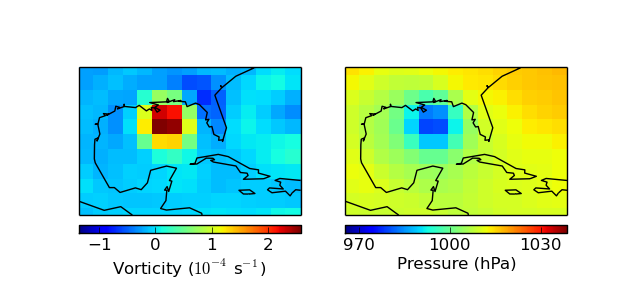
\includegraphics[width=\textwidth]{figures/galveston_1900-9-7_18-00_em0}
    \caption{Vorticity and pressure fields over the Gulf of Mexico from September the 7\ts{th}, 1900
        at 1800 UTC (taken from ensemble member 1). This shows the hurricane that would go on to hit
        Galveston, Texas. The hurricane is clearly visible in both the vorticity and pressure fields.}
    \label{fig:galveston}
\end{figure}

% In a more comprehensive study, \textcite{emanuel2010tropical} used an earlier version of the 20CR
% dataset to look at tropical cyclone activity from 1908-1958. He used dynamical downscaling (i.e.
% using a high resolution model with the 20CR data providing boundary conditions for this model, not
% to be confused with the simple cubic spline interpolation downscaling used in this study) to better
% represent the structure of the tropical cyclones. He found a ``marginally significant increase'' in
% the number of northern hemisphere tropical cyclones, along with a high correlation between the power
% dissipation index from derived from the 20CR reanalysis and the best tracks from the same period.

\section{IBTrACS Best Tracks Dataset}
\label{sec:ibtracs}
The International Best Track Archive for Climate Stewardship (IBTrACS)
\parencite{knappInternational2010} aims to be a homogenised global collection of best tracks of
tropical storms and tropical cyclones. It collects best tracks from numerous Regional Specialized
Meteorological Centers (RSMCs) and Tropical Cyclone Warning Centres (TCWCs), and combines these
together, removing duplicates and trying to detect common discrepancies, such as dates being different
by one day and the positions between tracks not being the same.

The dataset contains data for each track at 6 hourly time intervals (taken at 0000, 0600, 1200, 1800
UTC daily). It includes data on position, wind speed and pressure. It also includes information on
whether each individual point is a hurricane or not, and this information was used as part of the
classification process described in Section \ref{sec:classification}. It is split into separate
basins, and in this study only the North Atlantic (NA) basin will be used. The primary source of
data for this basin is the Atlantic Hurricane Database \parencite[HURDAT;][]{jarvinen1984tropical}.

% CULLED
% indeed there are ``no new storms in the NA or EP basins'' in the IBTrACS dataset.

Figure \ref{fig:hurr_per_year} shows the hurricane-timesteps per year, where a hurricane-timestep is
defined as being one individual recorded hurricane per 6-hour timestep in the best tracks database.
This means that one hurricane track over the course of the day counts as four hurricane-timesteps,
and if there are multiple hurricane tracks active in one timestep then each one will count towards
the total hurricane-timesteps. 

Following \textcite{vecchi2008estimates}, four historical eras are shown in this figure, henceforth
called the pre-Panama Canal (1890 - 1914), Panama Canal (1915 - 1943), aircraft reconnaissance (1944
- 1965) and satellite (1966 - 2009) eras.  These are of significance to the number of observed
hurricanes in the best tracks dataset. Before the opening of the Panama Canal, shipping was
mostly concentrated in the northern and eastern tropical Atlantic, and along the east coast of North
America. This meant that there were fewer ships in the Gulf of Mexico, an active hurricane area, and
consequently there is thought to be a gap in the recorded hurricanes in this period from this area.
The aircraft reconnaissance era lead to more detailed observations of hurricanes, although coverage
did not extend across the entire North Atlantic. Finally, after the advent of satellite technology,
the entire basin could be covered, and this began in 1966 \parencite{landsea2007counting}.

\begin{figure}[hb!]
    \centering
    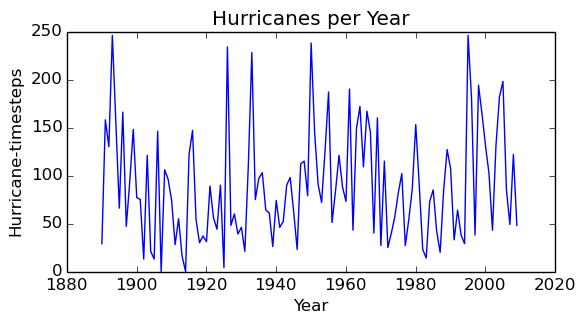
\includegraphics[width=\textwidth]{figures/hurr_per_year}
    \caption{Hurricane-timesteps from 1890 to 2009.}
    \label{fig:hurr_per_year}
\end{figure}

\newpage
Figure \ref{fig:yearly_hurr_dist} shows how the hurricanes are distributed over the course of a
year. Black dashed lines show the 1\ts{st} of June and the 1\ts{st} of December, and it is clear
that the vast majority of hurricanes (over 99\%) fall within this period. For this reason, only
dates that fell within this range were considered when detecting hurricanes in this study.

\begin{figure}[hb!]
    \centering
    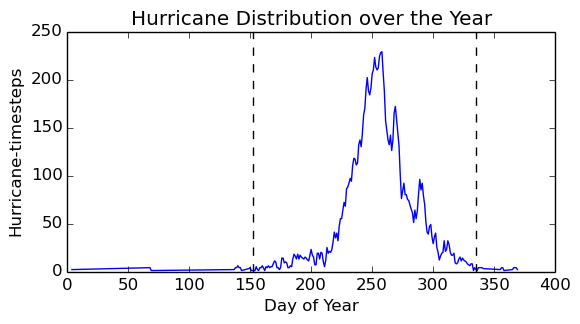
\includegraphics[width=\textwidth]{figures/yearly_hurr_dist}
    \caption{Hurricane distribution over the course of the year. The 1\ts{st} of June and the
    1\ts{st} of December are shown, these indicate the start and end of the analysis period in this
study. }
% CULLED: It can be seen that the vast majority of hurricanes fall within this period.
    \label{fig:yearly_hurr_dist}
\end{figure}

\chapter{Hurricane Detection Procedure}
\label{chap:hurricane_detection_proc}

% Overall description to go here, with flow chart.
% Mention:
% * project URLs
% * choice of tracking then classification vs classifying individual CDPs
% * amount of processing required

The hurricane detection procedure forms the basis of the rest of this study. It is a multi-step
procedure which logically follows the flowchart shown in Figure \ref{fig:hurricane_detection_proc}.
The procedure consists of separate steps, starting from the data in the 20CR and IBTrACS
datasets, and proceeding through the steps until detected hurricanes are found. 

\begin{figure}[ht!]
    \centering
    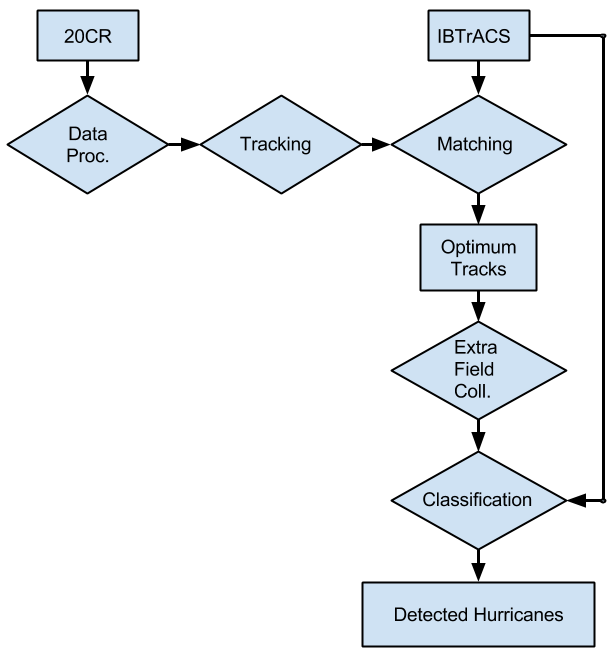
\includegraphics[width=0.7\textwidth]{figures/hurricane_detection_procedure}
    \caption{Flowchart showing the steps in the hurricane detection procedure. Processes are shown
    by diamonds, and data or results are shown by rectangles. }
    \label{fig:hurricane_detection_proc}
\end{figure}

\newpage
The computer code developed to perform these processes was all written in Python, apart from two
helper methods for calculating vorticity as in Section \ref{sec:vort}, which were written in C for
computational efficiency. The code for this project is all available at the following location:
https://github.com/markmuetz/stormtracks/. The code follows the structure set out in the flowchart
closely, with Python modules called c20data, tracking and matching. The Python project also contains
infrastructure code for allowing concurrent processing on the UCL computers, where the bulk of the
processing was done, following a simple master/slave pattern, with one computer designated as the
master, farming out jobs to multiple slave computers that would carry out the processing, whether it
be e.g. matching or extra field collection. 

There were constraints on the available disk space on the UCL computers, so the processing was
batched into decades, with the 20CR data for one decade downloaded, the processing run, and the
results gathered, before deleting that decade's data and moving onto the next one.  Bearing in mind
one decade's worth of 20CR data takes up about \SI{112}{GB} of disk space, downloading all of these
data and processing it took about 12 hours, even with the processing spread across multiple
computers. Therefore the complete run over the period from 1890 to 2009 took around six days. Given
that the processing was run on 12 computers, and accounted for roughly half of the 12 hours spent
for one decade, this represents around 36 days of processing time.

\section{Data Processing}

\subsection{Wind Fields and Vorticity}
\label{sec:vort}

% CULLABLE 250
In the 20CR data, the longitudinal and latitudinal wind fields, $u$ and $v$ respectively, were used
to calculate the vorticity and wind speeds. These are available at three different pressure levels:
Near Surface Pressure Level (NSPL), \SI{850}{hPa} and \SI{250}{hPa}. The \SI{250}{hPa} fields were
only used to determine whether or not they were suitable for tracking of hurricanes, and it was
found that they did not produce suitable tracks, and were not further used. The formula for
vorticity, $\omega$, is given by:

\begin{equation}
    \omega = \frac{\partial v}{\partial x} - \frac{\partial u}{\partial y}
    \label{eqn:vorticity}
\end{equation}

The surface of the earth, $R_e$, is taken as its mean radius of \SI{6371}{km}, and $\phi$, $\lambda$
denote the latitude and longitude coordinates in radians. $u_{i, j}$ denotes the longitudinal wind
speed at grid cell $i, j$. Then $\omega$ can approximated on the surface of the Earth using the
approximation: 

% Calculation in code is a little different because it uses degrees instead of radians:
% More like vorticity = du / (2 * dlon * cos(lat * pi / 180) * Earth_circ / 360) - dv / ((2 * dlat) * Earth_circ / 360)

\begin{equation}
    \omega \approx \frac{\Delta v}{2 \Delta x} - \frac{\Delta u}{2 \Delta y} = \frac{v_{i,j+1} - v_{i,j-1}}{2 R_e \cos{\phi} \Delta \lambda} - \frac{u_{i+1,j} - u_{i-1,j}}{2 R_e \Delta \phi }
    \label{eqn:vorticity_2nd_order}
\end{equation}

The vorticities at the NSPL and \SI{850}{hPa} levels were calculated.

\subsection{Maxima and Minima detection}
\label{sec:methods_maxima_minima}

For the vorticity fields, maxima are of primary interest as these represent grid cells where the
wind is rotating most strongly. Conversely, for the Pressure at Sea Level (PSL) field, minima are of
primary interest. A maximum or minimum was defined as a cell whose value was greater or less than
the value of all eight of its surrounding cells. Vorticity maxima play a vital role in deriving
tracks from the 20CR data, and pressure minima are useful both for comparison with the best tracks
data and classification of the tracks.

\subsection{Downscaling of Data}

The vorticity field was downscaled to a finer resolution. This was done to minimise the so called
``staircase effect'' \parencite{hodges1994general}, whereby tracks are seen to follow the grid cells
at the resolution of the 20CR data (an example of this ``staircase effect'' can be seen in Figure
\ref{fig:katrina_individual_match_em7}).  This downscaling was accomplished using a cubic spline
interpolation which takes into account the spherical nature of the globe, and the data were
downscaled to two and three times their original resolutions in both longitude and latitude, leading
to four and nine times the number of grid cells. The efficacy of this downscaling in improving the
position of the vorticity maxima will be demonstrated in Section \ref{sec:matching}.

% The vorticity field was downscaled to a finer resolution. This was done so as when tracks were
% derived from these data, the so called ``staircase effect'' \parencite{hodges1994general}, whereby
% tracks are seen to follow the grid cells at the resolution of the 20CR data, was minimised (an
% example of this ``staircase effect'' can be seen in Figure \ref{fig:katrina_individual_match_em7}).
% This downscaling was accomplished using a cubic spline interpolation, and the data were downscaled
% to two and three times their original resolutions. The efficacy of this downscaling in improving the
% position of the vorticity maxima will be demonstrated in Section \ref{sec:matching}.

\subsection{Data Processing Results}

Figure \ref{fig:katrina_data_proc} shows the progression of the data from its raw form, to a derived
vorticity, and then downscaled to three times the original resolution vorticity field. Figure
\ref{fig:katrina_max_mins} shows an example vorticity and pressure field taken from around Hurricane
Katrina, and the corresponding maxima for the vorticity and minima for the pressure fields.
The 2\textdegree\ resolution of the 20CR data is clearly visible in the middle figure. The more
precise location of the vorticity maximum can be seen in the right figure.

\begin{figure}[hb!]
    \centering
    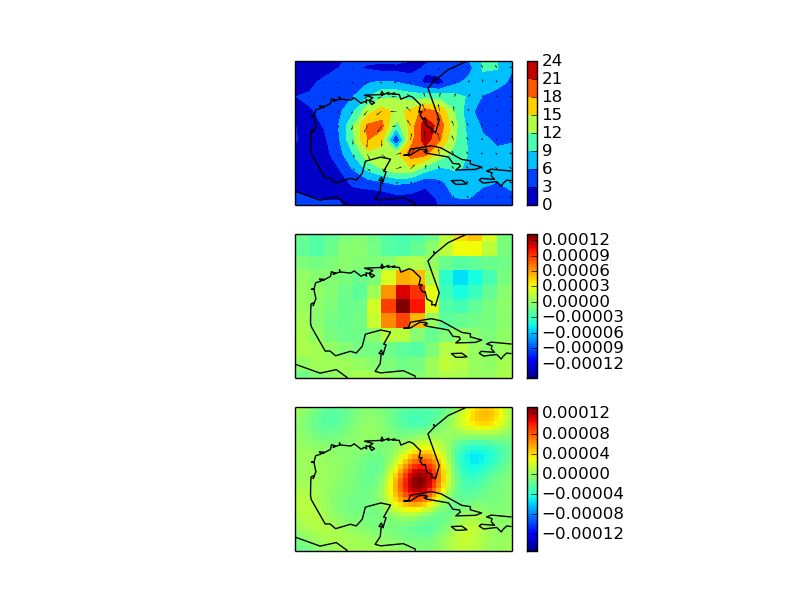
\includegraphics[width=0.9\textwidth]{figures/katrina_data_proc}
    \caption{Three different views of Hurricane Katrina over the Gulf of Mexico as it appears in the
        20CR on the 27\ts{th} August, 2005 at 1800 UTC (taken from ensemble member 1). The left
        figure shows the raw 20CR wind fields with contours fitted based on the wind speed. The
        middle figure shows the corresponding vorticity field. The right figure shows the data after
        they have been downscaled to three times the original resolution.}
    \label{fig:katrina_data_proc}
\end{figure}

\begin{figure}[hb!]
    \centering
    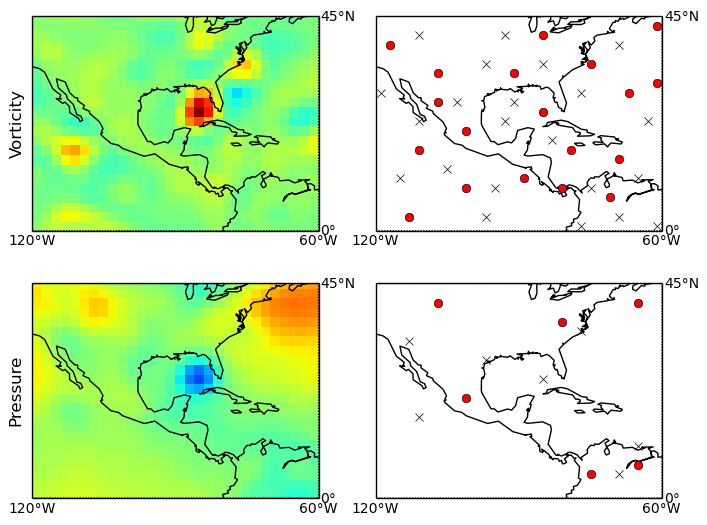
\includegraphics[width=0.9\textwidth]{figures/katrina_max_mins}
    \caption{Vorticity and pressure maximum and minimum detection as shown for Hurricane Katrina,
        on the 27\ts{th} August, 2005 at 1800 UTC (taken from ensemble member 1). Maxima are shown
        by red dots, and minima by black crosses. The large number of vorticity maxima should be
        noted, which is why a vorticity cutoff as described in Section \ref{sec:tracking} is
        employed. A clear vorticity maximum and pressure minimum can be seen indicating the position
        of Hurricane Katrina in this figure.}
    \label{fig:katrina_max_mins}
\end{figure}

\section{Tracking}
\label{sec:tracking}

From initial experimentation, it was found that tracking on minima of the pressure field did not
produce suitable tracks for identifying storm systems. This was due to the pressure field being
subject to synoptic scale disturbances that mean that minima may not be present due to the
surrounding synoptic gradient of this field. Whilst it is possible to apply high pass filtering to
remove these disturbances, it was decided to follow \textcite{reed1988evaluation,
thorncroft2001african} and produce derived tracks from the 20CR data based on vorticity maxima.

% TODOIMPROVE: This section is confusing on re-reading it. I think I need to make it clearer that I'm going to
% compare different configurations.
For each timestep, the vorticity maxima were calculated, as per Section
\ref{sec:methods_maxima_minima}. This was done for both the NSPL and \SI{850}{hPa} pressure
levels, and for the one, two and three times the actual 20CR resolution, yielding a total of six
possible configurations for the tracking. These various configurations were compared, and the
results can be seen in Section \ref{sec:matching}. Maxima that were below a cutoff value
of \SI{2.5e-5}{s^{-1}} were not used as part of the tracking algorithm, as these represent weak maxima
that are unlikely to be part of even tropical storms. 

% CULLED
% This is similar to the ``relaxed threshold
% criteria'' used in \textcite{camargo2002improving}.

The tracking algorithm used was a simple nearest neighbour tracking algorithm, with a modification
that counted two or more vorticity maxima that were sufficiently close as being part of the same storm
system, with the location and strength of the maximum given by the strongest of
these maxima. This cutoff distance was set as eight times the distance between the cells at
0\textdegree\ N, or approximately \SI{1800}{km}. This distance was found to reduce problems of
vorticity maxima merging and splitting. The algorithm worked as follows:

\begin{enumerate}
    \item Detect all vorticity maxima for the first timestep. If two maxima are less than the cutoff
        distance apart, combine both maxima, taking the strength and position of the strongest of
        the two maxima
    \item Make each of the vorticity maxima in the first timestep the beginning of a derived track
        % CULLED: (whose length could end up being only one)
    \item Detect all vorticity maxima in the second timestep, again combining close weaker maxima
        into stronger. 
    \item Calculate nearest neighbour in the second timestep to first timestep, and set this as the
        next member of the derived track
    \item Move onto the third timestep and repeat the process
\end{enumerate}

Whilst this algorithm is considerably less sophisticated that that of \textcite{hodges1994general},
it was found to produce sufficiently good tracks to pick up most of the best tracks in the IBTrACS
dataset, and almost all of the best tracks that were hurricanes (Section
\ref{sec:matching}). 

% CULLED: 
% A discussion of other tracking algorithms can be found in Section
% \ref{sec:discussion_tracking_algs}.

\section{Matching}
\label{sec:matching}

Once tracks have been derived from the 20CR, it is possible to match them to the corresponding best
tracks. The corresponding best track must be close the derived track in space, and its temporal
duration must overlap the duration of the derived track. In this project, an overlap of 6 timesteps,
or one and a half days, was required for there to be a match between a derived track and a best
track. Additionally, the mean distance from the derived track and the best track had to be lower
than a given threshold, taken as \SI{500}{km}. An example of a matching derived track taken from
one ensemble member and best track is shown in Figure \ref{fig:katrina_individual_match_em7}.
% N.B. em7 is counting from 0.
This shows how the cumulative and mean distances between a derived track (from ensemble member 8)
and a best track are calculated. All matching tracks across all the ensemble members for each of the
different configurations for Hurricane Katrina are shown in Figure
\ref{fig:katrina_six_tracking_configs}. Katrina started as a tropical depression to the East of
Florida, and then strengthened over the Gulf of Mexico, where it became a hurricane. This section of
the best track is particularly well matched in all of the figures, indicating that it is easier to
track hurricanes and stronger storms in general due to their more pronounced natures. The tighter
grouping of the higher resolution derived tracks around the best track can also be seen, indicating
that they may be providing a better track. 

\begin{figure}[hb!]
    \centering
    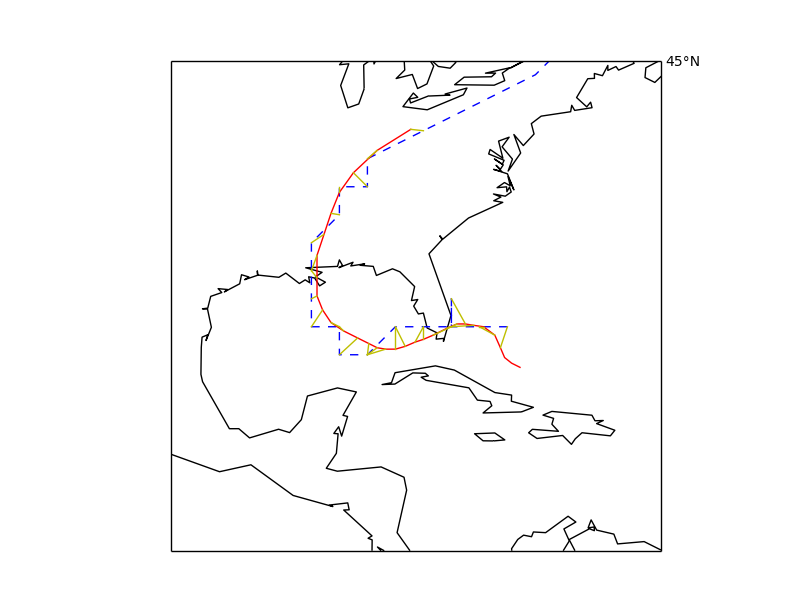
\includegraphics[width=\linewidth]{figures/katrina_individual_match_em7}
    \caption{Individual match between best track (red) and derived track (blue dashed) for Hurricane
        Katrina. The derived track was generated from the \SI{850}{hPa} pressure level using the
        original resolution and ensemble member 8. The match between the best track and the derived
        track is shown using yellow lines, which show the distance between the two tracks at each
        timestep. 
        % CULLED: The cumulative distance is the sum of these distances, and the mean distance is
        % the cumulative distance divided by the number of matches.
    }
    \label{fig:katrina_individual_match_em7}
\end{figure}

\begin{figure}[hbp]
    \centering
    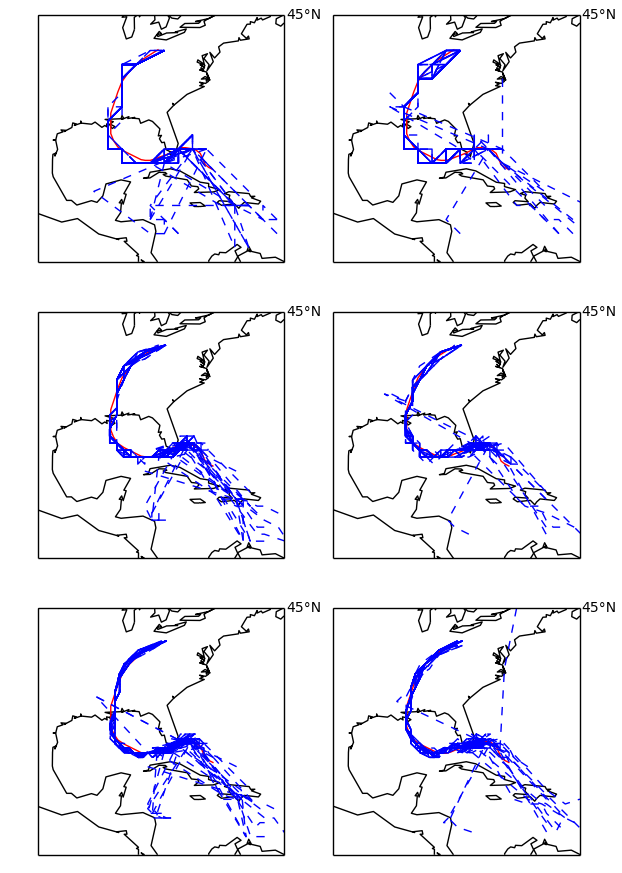
\includegraphics[width=4.5in]{figures/katrina_six_tracking_configs}
    \caption{The six different tracking configurations tested for their fit with the best track of
        Hurricane Katrina. Each of the individual figures shows all of the tracks across the
        different ensemble members that were matched with Hurricane Katrina.}
    \label{fig:katrina_six_tracking_configs}
\end{figure}

To judge the tracking ability of the different tracking configurations, this matching across all
best tracks and derived tracks was done for each year in the ten year period 2000-2009. For each
year, the cumulative distance between each derived track and best track across all ensemble members
was calculated. This number was divided by the total number of overlaps between derived tracks and
best tracks, so that a particular configuration that achieved relatively few matches would be
penalised. This produces a metric by which the various configurations can be judged, and each of
the configurations was then compared the others to see how they performed on this metric. 

The results of this comparison can be seen in Figure \ref{fig:tracking_wins_losses}. It is clear
that higher resolution, downscaled data produces better tracks that the unscaled data. This suggests
that for tracking, scaling of three times the original resolution should be used.

What is less clear is which is better: the NSPL or the \SI{850}{hPa} pressure levels. It is hard to
pick between them based on performance grounds on this metric alone. However, theoretical reasons
for preferring the \SI{850}{hPa} pressure level exist. These are that the vorticity at \SI{850}{hPa}
is less influenced by strong background flows, and therefore more suitable than the NSLP for
tracking of hurricanes \parencite{trigo2006climatology}. Due to the fact they are higher up, they are
also less affected by surface effects than the NSPL. Therefore the \SI{850}{hPa} level was chosen
over the NSPL. This has the added benefit of making comparison between this study and other studies
easer, as almost all other studies use the \SI{850}{hPa} pressure level, thereby allowing e.g.
comparison of the vorticity values found.

\begin{figure}[hbp]
    \centering
    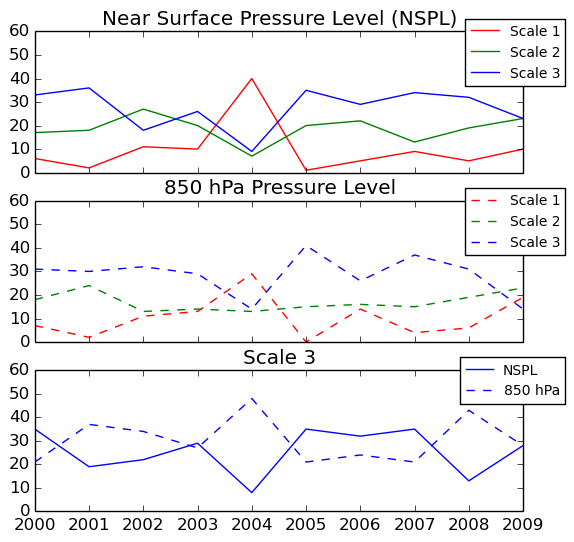
\includegraphics[width=\linewidth]{figures/tracking_wins_losses}
    \caption{Comparison for the number of wins/losses for each tracking configuration within the
        NSPL (top), the \SI{850}{hPa} pressure level (middle) and then the scale 3 groups. In both
        of the pressure level comparisons it is clear that the scale 3 configuration comes out on top,
        with eight wins in both cases. The comparison between scale 3 for the two pressure levels is less
        clear, with each configuration winning five times apiece.}
    \label{fig:tracking_wins_losses}
\end{figure}

\newpage
\section{Extra Field Collection}
\label{sec:extra_field_collection}

Up until this point in the processing, only the $u$ and $v$ wind fields at different pressure levels
have been utilised. From these, the vorticity has been calculated and tracks have been derived from
the maxima of these fields. However, to successfully classify part of a track as being of hurricane
strength, it is necessary to collect more fields. These fields will help to distinguish hurricanes
from non-hurricanes. To this end, the latitude, longitude, date and ensemble member were used to
obtain further variables from the 20CR dataset. These variables were:

\begin{enumerate}
   \item \textbf{Vorticity:} the value of the vorticity at the local maximum.
    \item \textbf{Minimum pressure:} the pressure minimum within \SI{1000}{km} of the vorticity
        maximum.
    \item \textbf{Distance to minimum pressure:} the distance from the vorticity maximum to the
        pressure minimum.
    \item \textbf{Ambient pressure difference:} the difference in pressure between the minimum
        pressure and the local mean pressure, as calculated by taking the surrounding 121 grid cells
        and averaging their pressures.
    \item \textbf{Temperature at NSPL:} the temperature at the height of the NSPL.
    \item \textbf{Temperature at \SI{850}{hPa}:} the temperature at the height of the \SI{850}{hPa}
        pressure level.
    \item \textbf{Temperature difference:} the temperature difference between the NSPL and
        \SI{850}{hPa} pressure levels.
    \item \textbf{Maximum wind speed:} the maximum wind speed in the nearest 121 grid cells as taken
        from the \SI{850}{hPa} pressure level.
    \item \textbf{Distance to maximum wind speed:} the distance (in km) from the vorticity
        maximum to the wind speed maximum.
    \item \textbf{Direction to maximum wind speed:} the angle (in radians) from the vorticity
        maximum to the wind speed maximum.
    \item \textbf{Convective available potential energy:} a measure of atmospheric instability.
    \item \textbf{Atmospheric water vaopur content:} amount of water vapour held by the atmosphere.
        % CULLED:
    % \item \textbf{Relative humidity at the NSPL:} Initial experimentation showed that this field was
        % not useful for hurricane detection so it was not collected for all years.
\end{enumerate}

Figure \ref{fig:katrina_best_derived_comparison} shows the derived pressure and maximum wind speed
for Katrina, plotted with the equivalent variables for the matching best track. From this figure, it
is clear that there is far more range in both pressure and maximum wind speed for the best
track than there is for the derived track. This is to be expected, as the 20CR data is at a
resolution that will reduce the relative values of e.g. the maximum wind speed, as discussed in
\textcite{walsh2007objectively}. However, to more fully test this, the values of all pressures and maximum wind
speeds for all ensemble members was plotted against the corresponding best track pressures and
maximum wind speeds as is shown in Figure \ref{fig:press_max_ws_corr_2005}. This figure shows that
the best track pressure is shown to vary far more than the derived track pressure, exhibiting a much
larger lowest possible value. The best track maximum wind speed is also shown to vary more,
exhibiting a much larger maximum wind speed. Only weak correlation is seen for both the vorticity
and the maximum wind speed.

\begin{figure}[hb!]
    \centering
    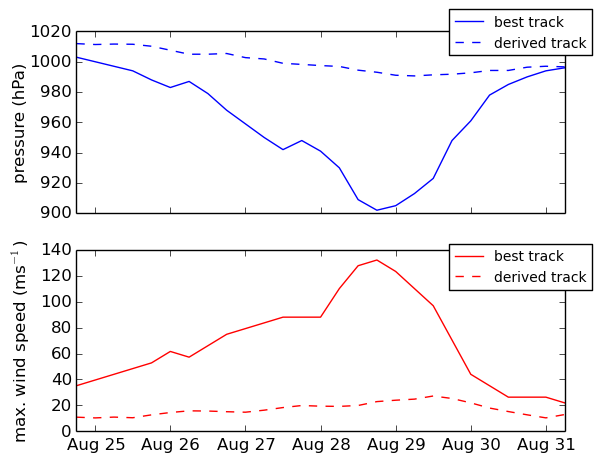
\includegraphics[width=\textwidth]{figures/katrina_best_derived_comparison}
    \vspace{-10pt}
    \caption{Time series graphs taken from Hurricane Katrina (2005), showing pressure and maximum
            wind speed taken from the best track for Katrina and the corresponding pressure from derived
            track (taken form ensemble member 8). }
    \label{fig:katrina_best_derived_comparison}
    \vspace{-10pt}
\end{figure}

\begin{figure}[ht!]
    \centering
    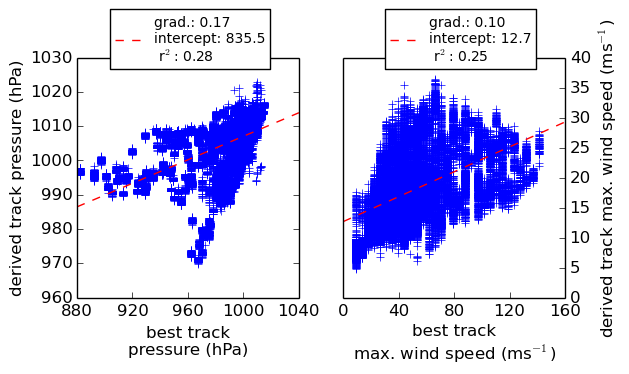
\includegraphics[width=\textwidth]{figures/press_max_ws_corr_2005}
    \vspace{-10pt}
    \caption{Correlation of best track and derived track pressures and maximum wind speeds. The
        $r^2$ values indicate that there is weak some correlation between these variables. }
    \label{fig:press_max_ws_corr_2005}
\end{figure}

\newpage
\section{Classification}
\label{sec:classification}

% Description of the goal of classification and how it applies in this setting. Set out terminology
% that I am going to use.
% standard by which the various classifiers can be trained/judged.
Now that for each ensemble member a number of tracks have been derived from the 20CR data, and that
extra fields have been collected using the tracks' positions at different timesteps, it is possible
to use this information to classify each point of each track as either being a hurricane or not.
These points will be knows as cyclone data points (CDPs) and for a typical year there are around
\SI{100000}{} of these points, spread across the 56 ensemble members.

% TODO: definition of classification.
Classification is the process of taking a dataset and splitting it up into various categories based
on the attributes of each item in the dataset. For the purposes of hurricane classification, this is
a binary classification, i.e. a CDP is either a hurricane or it is not. More fine-grained approaches
are possible, such as splitting each CDP into a category from the Saffir-Simpson hurricane scale
\parencite{simpson1974hurricane}, but in this analysis the only concern was trying to correctly
categorise whether or not a given CDP was a hurricane. In classification terminology, each CDP
represents one sample, and the different fields for each CDP are known as features for that sample.

Given that each derived track has also been matched to a best track, it is also possible to use the
information from the best tracks dataset about whether the point on the best track is a hurricane or
not as an objective standard for whether or not the corresponding point on the derived track
represents a hurricane. This is represented visually in Figure \ref{fig:cdp_2005_with_hurrs}, which
shows every CDP for 2005, as well as whether the individual point has been matched to a
hurricane in the best tracks dataset or not. Missed hurricanes are hurricanes which are present in
the best tracks database, but which were not in the CDP for the derived track. 
There were relatively few of these, around 4\% over the years 1990 to 2009. 

In classification terminology, this matching of CPDs to hurricanes represents the gold standard by
which the classification algorithms can be trained, and by which their performance can be validated.
Once the classifiers have been trained, and their performance validated, they can then be used to
classify new data based on the training they have undergone. This training process, where features
from a set of samples are matched against a gold standard, is known as supervised machine learning.

% CULLED:
% This is in contrast to other types of machine learning where there is no objective gold standard by
% which to train the algorithms, known as unsupervised machine learning. An example of unsupervised
% machine learning can be seen in \textcite{studholme2014objective}, where a K-means clustering
% algorithm is used to determine the extratropical transition of cyclones.

\begin{figure}[hb!]
    \centering
    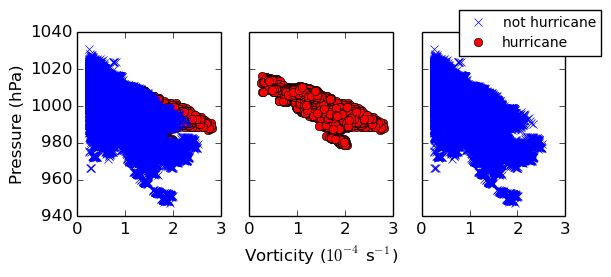
\includegraphics[width=\textwidth]{figures/cdp_2005_with_hurrs}
    \vspace{-10pt}
    \caption{Every CDP from all ensemble members for the year 2005, as well as indication of whether
        the CDP was matched to a hurricane (red circle) or not (blue cross). The difference between
        the top row (Pressure - Vorticity) and the bottom row (Temperature at \SI{850}{hPa} -
        Vorticity) shows that some hurricanes may be distinguishable from non-hurricanes when
        looking at one variable, but not another. For both rows, the middle and right figures show the
        overlap between the two sets.}
    \label{fig:cdp_2005_with_hurrs}
\end{figure}

\subsection{Classification Successes and Errors}
\label{sec:cla_successes_and_errors}

% Explanation of FPs and FNs, TPs and TNs. Talk about Gold standard and how I am using IBTrACS as a
% gold standard. Relationship to Type I/II errors (maybe). Venn diagram showing FP/FN/TP/TN.
When classifying data with a binary classifier for which a gold standard exists, there are four
possible results of an individual classification. These are:

\begin{enumerate}
    \item \textbf{True Positive (TP):} The classification predicts that the CDP is a hurricane and
        this is verified by the best tracks information.
    \item \textbf{True Negative (TN):} The classification predicts that the CDP is not a hurricane
        and this is verified by the best tracks information.
    \item \textbf{False Positive (FP):} The classification predicts that the CDP is a hurricane and
        this is refuted by the best tracks information.
    \item \textbf{False Negative (FN):} The classification predicts that the CDP is not a hurricane
        and this is refuted by the best tracks information. Missed hurricanes are also added to this
        number.
\end{enumerate}

When classifying a dataset, the collection of these results can be represented visually with a Venn
diagram, as shown in Figure \ref{fig:tf_np_venn}. They can also be represented in tabular form in an
Error Matrix. An example of an Error Matrix
can be seen in Table \ref{tab:tf_np_table}, which shows the successes and failures of a simple
classifier for a subset of the data.

% CULLED: (also called a Contingency Table or Confusion Matrix)

\begin{figure}[hb!]
    \centering
    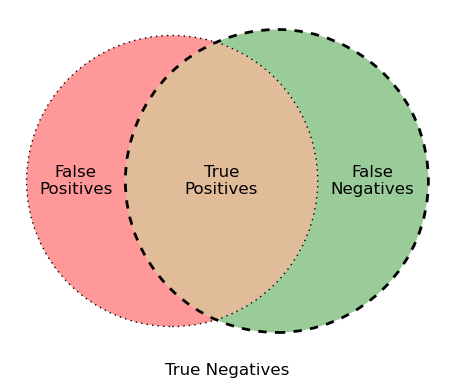
\includegraphics[width=0.6\textwidth]{figures/tf_np_venn_cropped}
    \vspace{-10pt}
    \caption{Venn diagram showing relationship of True Positives, False Positives, True Negatives and
        False Negatives. Everything inside the thick dashed line is objectively true, as determined
        by the gold standard. Everything inside the thin dotted line is predicted to be true, by the
        classification algorithm. The intersection of these two sets represents all True Positives.}
    \label{fig:tf_np_venn}
    \vspace{-10pt}
\end{figure}

\begin{table}[ht!]
    \centering
    \begin{tabular}{ l | c c }
                                & Condition Positive & Condition Negative \\
        \hline
        Classification Positive & \SI{40587}{} & \SI{14344}{} \\
        Classification Negative & \SI{23125}{} & \SI{2042954}{} \\
    \end{tabular}
    \caption{Error Matrix showing the number of True Positives, False Positives, False Negatives and
        True Negatives for the training run with the Stochastic Gradient Descent classifier described
        later in this section. }
    \label{tab:tf_np_table}
\end{table}

\newpage
\subsection{Sensitivity, Positive Predictive Value and False Positive Rate}

From the success and error results, various metrics are defined that give a measure of how well a
particular classifier performs at various tasks. Of these metrics, three will be utilised in this
project:

\begin{enumerate}
    \item \textbf{Sensitivity:} This is defined as $\frac{TP}{TP + FN}$. It gives a measure of how
        many hurricanes are correctly detected from all the actual hurricanes. 1 represents a
        perfect sensitivity.
    \item \textbf{Positive Predictive Value (PPV):} This is defined as $\frac{TP}{TP + FP}$. It
        gives a measure of how many of the predicted hurricanes from the classification algorithm
        are actually hurricanes. 1 represents a perfect PPV.
    \item \textbf{False Positive Rate (FPR):} This is defined as $\frac{FP}{FP + TN}$. It gives a
        measure of the detection rate of all actual hurricanes. 0 represents a perfect FPR.
\end{enumerate}

Sensitivity is often plotted against FPR to make a Receiver Operator Characteristic (ROC)  plot.
ROC plots are useful for determining which particular classifier is considered to perform best over
a given training and validation dataset. The top left corner of this plot represents perfect
classification. Another plot which will be used in this project is a plot of Sensitivity against
PPV, which will again be used to determine which of the classifiers performs best. This plot is more
useful in the context of this project, as for the given datasets, very high values of FP detection
are seen, which means that the FPR will typically be very low, and less information can be gleaned
from this particular metric. Also, as will be explained in the next section, the Sensitivity and the
PPV can be used to obtain an estimate of the number of actual hurricanes. Examples of these plots
can be seen in Figure \ref{fig:ppv_and_fpr_vs_sens}.

For the values in Table \ref{tab:tf_np_table} the values would be:

\begin{table}[hb!]
    \centering
    \begin{tabular}{ l l }
        Sensitivity: & \SI{0.637}{} \\
        PPV: & \SI{0.739}{} \\
        FPR: & \SI{6.97e-3}{} \\
    \end{tabular}
    \label{tab:success_metric_table}
\end{table}

\subsection{Estimate of the Number of Actual Hurricanes}
\label{sec:estimated_hurricanes}

When any of the classifiers is run on a dataset, it will produce a prediction of which of the
members of that dataset are hurricanes, $H_{predicted}$. The PPV value derived for that particular classifier will
allow an estimate of the number of TPs for that prediction. Likewise, from the estimated number of
TPs, the sensitivity will allow a means of estimating the number of actual hurricanes, $H_{estimated}$,
in the dataset. The equation for this is:

\begin{equation}
    H_{estimated} = \frac{PPV \times H_{predicted}}{sensitivity}
    \label{eqn:n_actual_hurricane}
\end{equation}

\subsection{Classifiers}

% TODO: 1/2 sentences saying what is in this section.

\subsubsection{Threshold Classifier}
% How this is related to a Decision Tree classifier, how it was optimised.
The threshold classifier is the simplest of the classifiers considered. It works by using different
values for thresholds for one or more of the collected fields for each CDP. Any CDPs which have
field value which are e.g. higher than the specified threshold are considered hurricanes, and any
which are lower or equal to the threshold are considered not hurricanes. Despite its simplicity,
good results are possible with the threshold classifier by judicious choice of the thresholds for
each of the fields. 

These thresholds were first picked manually, then a simple brute force search was carried out for
values on either side of the chosen values. The metric for success was the sum of the sensitivity
and the PPV for the given classifier, where a larger value is better (a value of 2 would be perfect
for this metric). It is also very easy to configure this classifier so as to increase either the
sensitivity or PPV, although there is a trade-off between these two metrics, as shown in Figure
\ref{fig:threshold_sens_ppv_vort}. The optimum values for these thresholds are shown in the
Table \ref{tab:threshold_values}. The other fields that were collected, such as the convective
available potential energy, were not found to significantly improve the performance of this
classifier.

\begin{table}[hb!]
    \centering
    \begin{tabular}{ l l }
        Vorticity: & \SI{10.4e-5}{s^{-1}} \\
        Maximum wind speed: & \SI{16.1}{ms^{-1}} \\
        Temperature at NSPL: & \SI{297.2}{K} \\
        Temperature at \SI{850}{hPa}: & \SI{286.7}{K} \\
        Ambient pressure difference: & \SI{563.4}{hPa} \\
    \end{tabular}
    \caption{Optimum threshold values.}
    \label{tab:threshold_values}
\end{table}

This classifier is a simple version of a decision tree classifier, which passes the incoming data
through a series of binary tests, determining which category a particular CDP should end up in based
in the results of these tests.

The approach of using thresholds is very similar to the approach taken by
\textcite{walsh1997objective}. The main difference between his approach and the one here is that in
this case the thresholds are applied after the processing has been done, thereby allowing far more
scope for experimenting with changes to these threshold values (i.e. the whole processing step does
not have to be run to experiment with different threshold values). This allows for a much faster
retrieval of optimum thresholds with regard to a given metric, although it comes at a cost of having
to run the data analysis in a way that gathers fields for all of the CDPs without being able to
discard CDPs based on whether or not they pass a particular threshold test.

\begin{figure}[ht!]
    \centering
    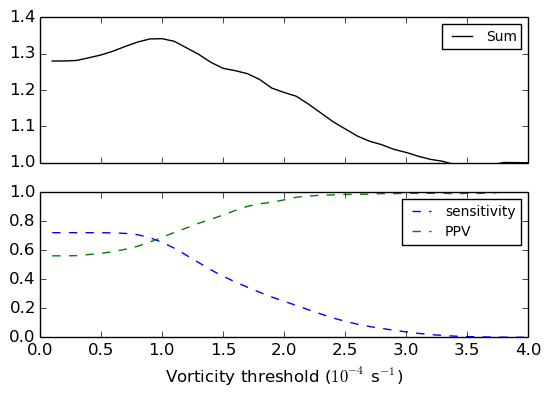
\includegraphics[width=\textwidth]{figures/threshold_sens_ppv_vort}
    \vspace{-10pt}
    \caption{Sensitivity and PPV are shown to vary with the vorticity threshold used for a threshold
        classifier (bottom). Their sum is shown in the top graph. For low vorticity threshold, high
        sensitivities are seen (because there are fewer FNs) and lower PPVs are seen (as there are
        many FPs). As the threshold increases, the sensitivity decreases and the PPV increases as
        the FNs increase and the FPs decrease. Their sum shows a clear maximum around the
        intersection of the two individual lines, at a vorticity value of \SI{1e-4}{s^{-1}}. All
        other threshold values are the same as in Table \ref{tab:threshold_values}. }
    \label{fig:threshold_sens_ppv_vort}
\end{figure}

\subsubsection{Linear/Quadratic Discriminant Analysis Classifiers}

% How these work.
For binary classification, Linear Discriminant Analysis (LDA) and Quadratic Discriminant Analysis
(QDA) are two closely related classification algorithms that allow computationally cheap
classification of data where a gold standard is available under trained supervision.
\textcite{mclachlan2004discriminant} gives a full account of both approaches, and a brief description of how they
work will be given here. The principal idea is to calculate the mean and covariance for all the
features of each group of data: $\mu_1$, $\sigma_1$ and $\mu_2$, $\sigma_2$. $\mu_1$ will lie at the
heart of the first group of features, and $\sigma_1$ will give a measure of the spread of this group
amongst each of the feature axes, and likewise for the second group. LDA then finds the dividing
surface between the two means (a plane in the same number of dimensions as there are features) based
on the relative values of the two variances. QDA is similar except that the dividing surface is
governed by a quadratic equation, and thus affords greater discriminating power between the two
groups.

The implementations of these algorithms in the Python library scikit-learn were used
\parencite{scikitLearn2011}.

\subsubsection{Stochastic Gradient Descent Classifiers}
% How this works. Its relation to SVM.
Stochastic Gradient Descent (SGD) classifiers are an efficient class of classifiers that can scale
to 2 million samples, and are thus suitable for the problem in this project
\parencite{shalevshwartz07pegasos, bottou2008tradeoffs}. This makes them more suitable than e.g. a Support
Vector Machine (SVM) classifier \parencite{cortes1995support}, to which they are closely related.
SVM classifiers typically only scale to around \SI{10e5}{} samples and therefore would not scale to
the number of samples used in this study. To understand the essentials of how an SGD classifier
works, it is useful to consider how an SVM classifier works first.

SVM classifiers work by calculating the hyperplane or set of hyperplanes which separate the two
categories into two distinct groups with the clearest possible gap between them. In the case where
there is no clean divide between the two categories, SVM classifiers will pick the hyperplanes which
most cleanly divide them \parencite{cortes1995support}. By use of the kernel trick
\parencite{aizerman1964theoretical}, SVM classifiers are not restricted to linear division between
the categories, but can represent more complex surfaces than just hyperplanes. The locations of the
hyperplanes which best separates the samples are calculated analytically.

SGD classifiers use the same underlying idea of hyperplanes to split the samples into two distinct
categories, however instead of calculating the location of the hyperplanes analytically, their
position is found iteratively using an SGD algorithm for optimising the position of this hyperplane.
This allows SGD classifiers to scale to far more samples than their SVM counterparts, whilst still
solving the same underlying problem (albeit possibly less optimally).

Again, the scikit-learn implementation for this classifier was used \parencite{scikitLearn2011}.

% CULLED:
% This particular classifier is sensitive to feature scaling, which is where a larger absolute range
% for e.g. pressure than vorticity leads to the classification being unduly biased towards this
% feature. Therefore the input features must be scaled before the classifier is trained with this
% dataset, and likewise any data to be classified must be scaled using this same scaling as was used
% for the training dataset. Dataset scaling was provided by the scikit-learn library.

% CULLED
% \subsubsection{Combining Classifiers}
% With some of the classifiers, it was clear from examination of the output that they performed well
% apart from producing FPs in areas of e.g. low vorticity or low temperature at \SI{850}{hPa}.
% Therefore it made sense to use e.g. an SGD classifier in conjunction with a threshold classifier.
% The result of this is to reduce the number of FPs, and increase the number of TNs by the same
% amount. This has the effect of increasing the PPV and FPR, but at the expense of the sensitivity.

\subsection{Classifier Performance}

% TODO lead in sentence.
% Figures showing performance of various classifiers in terms of FP/FN/TP/TN for 3 variables plotted
% against vorticity for training set. Discussion of performance differences.

% Explain how 20 years worth of data were split into a training/validation dataset.
\subsubsection{Training Dataset}
\label{sec:training_dataset}
For the training dataset, all tracks from all ensemble members from the even years between 1990 and
2008 were taken. Given that each track is comprised of multiple (at least six) CDPs, this leads to a
large number of samples. On average, there were \SI{211906}{} samples per year, leading to a total
sample size of 2.12 million samples. This training dataset was used as a way of picking optimum
values for the threshold classifier manually (as defined by a maximum combined value of sensitivity
and PPV), and then using a brute force around the chosen values to verify that these values were
indeed the local maximum. The training dataset was also used to train each of the LDA, QDA and SGD
classifiers.

\subsubsection{Validation Dataset} 
The validation dataset was similarly made up of all the tracks from all ensemble members from the
odd years between 1991 and 2009. This ensured that the training and validation datasets were
independent, yet still spanned the almost the same time period. It had a similar number of samples
as the training dataset: 2.14 million samples.

\subsubsection{Performance Metrics}

From the performance metrics shown in Table \ref{tab:classifier_performance_metrics} and Figure
\ref{fig:ppv_and_fpr_vs_sens}, there is clearly some difference in performance between the different
classifiers. The LDC classifier performs least well on on sensitivity, and poorly on PPV, therefore
it is not deemed suitable for classification in this context. The QDC categoriser performs
particularly well on sensitivity, but is worst for PPV and FPR. This does not preclude its use for
classification; if it were important to not miss as many hurricanes as possible, and a high number
of FPs was acceptable, than it may be a suitable classifier. The two
remaining classifiers, the threshold and the SGD, perform similarly well on sensitivity, but the SGD
classifier outperforms the threshold classifier on the PPV, therefore it is chosen as the classifier
to use.

% CULLED:
% Indeed, coupled with a threshold
% classifier (``QDC/Thresh.''), it performs well on both sensitivity and PPV metrics. 

\begin{figure}[hb!]
    \centering
    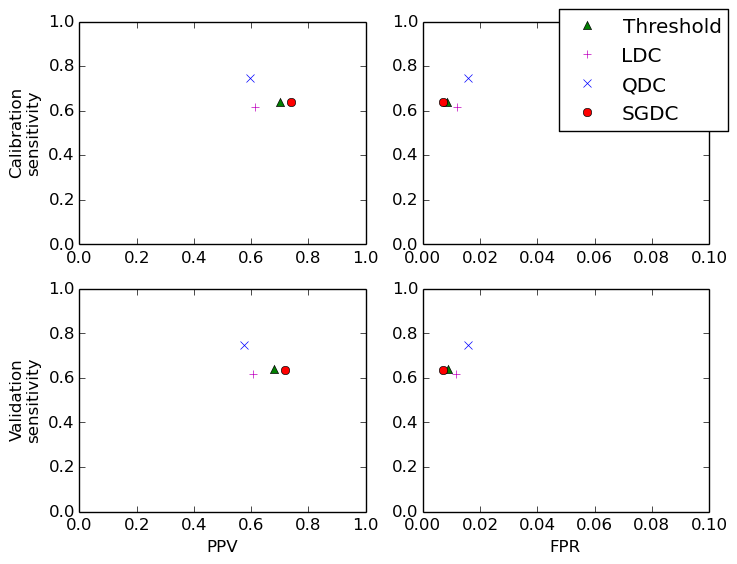
\includegraphics[width=\textwidth]{figures/ppv_and_fpr_vs_sens}
    \caption{Classifier performance shown for training (top) and validation (bottom) datasets,
        showing PPV vs sensitivity (left) and FPR vs sensitivity - Receiver Operating Characteristic
        plot (ROC plot, right). Note that x-axis on the ROC plots only goes from 0 to 0.1. }
    \label{fig:ppv_and_fpr_vs_sens}
\end{figure}

\begin{table}[hb!]
    \centering
    \begin{tabular}{ l | l l r | l l r | }
        \cline{2-7}
        & \multicolumn{3}{c |}{Training} & \multicolumn{3}{c |}{Validation} \\
        & \multicolumn{1}{c}{Sens.} & \multicolumn{1}{c}{PPV} & \multicolumn{1}{c|}{FPR} &
            \multicolumn{1}{c}{Sens.} & \multicolumn{1}{c}{PPV} & \multicolumn{1}{c|}{FPR} \\
        \hline
% cal: 0.6385453289804118, 0.702436244971252, 0.008377007122935034, 
% val: 0.6702334298858409,0.6811546520286066, 0.008826099523583321
        \multicolumn{1}{|c|}{Threshold} & 0.639 & 0.702 & \SI{8.38e-3}{} & 0.670 & 0.681 & \SI{8.82e-3}{} \\
% cal: 0.6177172275238574, 0.6129645204498022, 0.012078950156953441
% val: 0.6312659737604361, 0.6053164722412835, 0.011579432259338635
        \multicolumn{1}{|c|}{LDC} & 0.618 & 0.612 & \SI{12.08e-3}{} & 0.631 & 0.605 & \SI{11.58e-3}{} \\
% cal: 0.7484618282270216, 0.5963358969549177, 0.015689997268261573
% val: 0.7647299369568922, 0.5755725973992665, 0.015864258395292107
        \multicolumn{1}{|c|}{QDC} & 0.748 & 0.596 & \SI{15.69e-3}{} & 0.765 & 0.576 & \SI{15.86e-3}{} \\
% cal: 0.6370385484681065, 0.7388724035608308, 0.006972251953776264
% val: 0.6369398534673709, 0.7170643750479552, 0.007070274695750501
        \multicolumn{1}{|c|}{SGDC} & 0.637 & 0.739 & \SI{6.97e-3}{} & 0.640 & 0.717 & \SI{7.07e-3}{} \\
% cal: 0.6629363385233551, 0.6684761965054444, 0.010181801566909607 
% val: 0.6819219628556824, 0.6619035805838088, 0.009799161057981525
        % CULLED: \multicolumn{1}{|c|}{QDC/Thresh.} & 0.663 & 0.668 & \SI{10.18e-3}{} & 0.682 & 0.662 & \SI{9.79e-3}{} \\
        \hline
    \end{tabular}
    \caption{Performance metrics for each of the classifiers.}
    \label{tab:classifier_performance_metrics}
\end{table}

\chapter{20\ts{th} Century Analysis Results}
\label{chap:results_analysis}
% Data analysis and results.

\section{Hurricane Frequencies Over the 20\ts{th} Century}
\label{sec:hurr_freq}

Figure \ref{fig:20th_century_hurricane_timesteps} shows a comparison of the number of
hurricane-timesteps (as defined in Section \ref{sec:ibtracs}) taken from the IBTrACS dataset, and
calculated from the 20CR dataset. To calculate the estimate for the number of hurricane-timesteps
(henceforth ``estimated hurricane-timesteps''), the detection procedure was run over each year of
the period from 1890 to 2009, and for each ensemble member. This was used to work out a value for
the predicted number of hurricane-timesteps for each year, with one value per ensemble member. The
sensitivity and PPV from the years 1990 to 2009 (the training and validation period combined) were
used in the formula given in Section \ref{sec:estimated_hurricanes}, to give the estimated
hurricane-timesteps for each year. This was done by multiplying each predicted number of
hurricane-timesteps by the PPV divided by the sensitivity, or a factor of $\frac{0.728}{0.637} =
1.143$ . The maximum and minimum numbers of estimated hurricane-timesteps in any ensemble member
were used to plot the light blue area, and the mean of the ensemble members was plotted using the
blue dashed line.

For the results of this chapter it is useful to use the four eras described in Section
\ref{sec:ibtracs}. These were the pre-Panama Canal (1890 - 1914), Panama Canal (1915 - 1943),
aircraft reconnaissance (1944 - 1965) and satellite (1966 - 2009) eras. Results will be presented
with reference to these eras.

From the top graph in Figure \ref{fig:20th_century_hurricane_timesteps}, there is clearly a marked
correlation between the two time series. There is also a suggestion of a discrepancy between the two
time series in the pre-Panama Canal era and the aircraft reconnaissance era, with the estimated
hurricane-timesteps being greater in the pre-Panama Canal era, and fewer in the
aircraft reconnaissance era. This is borne out by the bottom graph in Figure 
\ref{fig:20th_century_hurricane_timesteps}, which shows the best tracks hurricane-timesteps minus the
estimated hurricane-timesteps. Here there is a clear sign that the best tracks hurricane-timesteps
is substantially lower than the estimated hurricane-timesteps in the pre-Panama Canal era. It is
also evident that the best tracks hurricane-timesteps is substantially larger in the aircraft
reconnaissance and early satellite eras.

\begin{figure}[ht!]
    \centering
    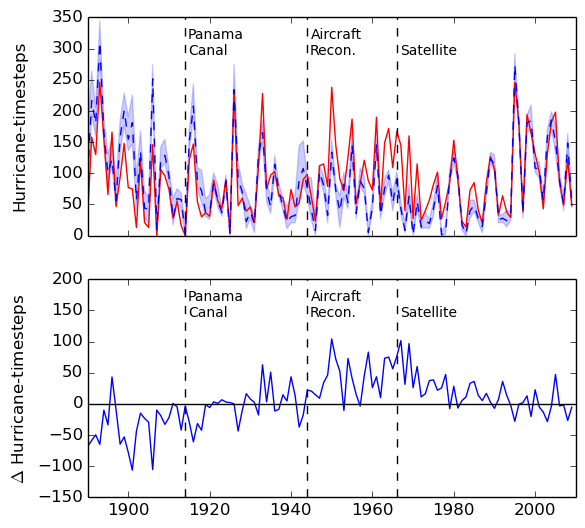
\includegraphics[width=\textwidth]{figures/20th_century_hurricane_timesteps}
    \caption{(top) The hurricane-timesteps per year as taken from the IBTrACS best tracks database
        (red), and the mean across ensemble members of the estimated values taken from the 20CR
        dataset (blue dashed). The blue shaded range shows the difference between the maximum and maximum
        taken from the ensemble members. The division between four eras: pre-Panama Canal, Panama
        Canal, aircraft reconnaissance and satellite are shown with dashed black vertical lines.
        (bottom) The estimated value subtracted from the best tracks value for each year. 
        % CULLED: A negative value means that the estimation is larger than the best tracks value.
    }
    \label{fig:20th_century_hurricane_timesteps}
\end{figure}

\newpage
Figure \ref{fig:20th_century_hurricane_corr} shows the correlation of the two time series, first
over the whole of the time period, and second by splitting the time period into two roughly equal
periods, based on the start of aircraft reconnaissance (1944). Given the high $r^2$ value of
\SI{0.63}{} shown in the first correlation plot, these series are very well correlated. The gradient
is less than unity though, which implies that there are fewer estimated hurricane-timesteps than
there are best tracks hurricane-timesteps over the whole period (although this effect is slightly
reduced by the positive y-intercept). From analysing the two time periods separately, as in the
second correlation plot, a clear distinction between the two periods can be seen, with the pre-1944
estimated numbers clearly estimating more hurricanes than were seen in the best tracks database, and
the reverse being true in the post-1944 period. The pre-1944 period has a gradient of \SI{1.04}{}
and a y-intercept of \SI{15.31}{}. The post-1944 period has a slop of \SI{0.83}{} and a y-intercept
of \SI{-8.52}{}.

\begin{figure}[hb!]
    \centering
    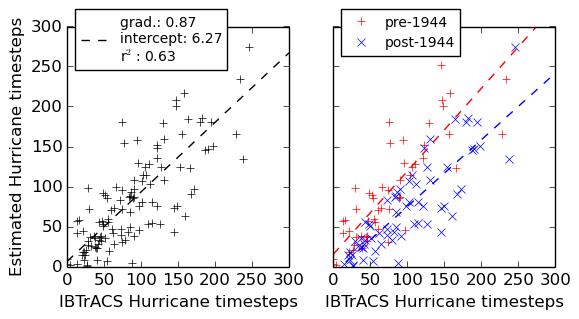
\includegraphics[width=\textwidth]{figures/20th_century_corr}
    \caption{Correlation plots showing the whole of the 20\ts{th} century (left) and splitting the
    20\ts{th} century into pre-1944 and post-1944 (right). From the left plot, the high value for
    $r^2$ indicates good correlation between the two time series. From the right plot, the different
    gradients of the lines of best fit indicate that in the pre-1944 period the estimated tracks
    were on average higher than the best tracks, and in the post-1944 period the estimates tracks were
    lower. }
    \label{fig:20th_century_hurricane_corr}
\end{figure}

\newpage
\section{Hurricane Frequencies in each Era}
\label{sec:hurr_freq_in_each_era}
Figure \ref{fig:20th_century_hurricane_corr_split} shows a finer breakdown of the two series based
on the four eras. The values of $r^2$ range between 0.68 to 0.80, meaning there is good correlation
between the two time series within each era. This figure again shows that the number of estimated
hurricane-timesteps in the pre-Panama Canal era is far higher than in the best tracks database, both
due to the large positive y-intercept and the gradient which is greater than unity. Reasons for this
are discussed in Section \ref{sec:freq_comparison}. In the Panama Canal era, the gradient is
slightly below unity, and the y-intercept is small and positive, which means that the two time
series are well matched. The most surprising era is the aircraft reconnaissance era, for which the
gradient is substantially less than unity, and the y-intercept is very close to zero. This means
that during the aircraft reconnaissance era, the estimated hurricane-timesteps were almost always
lower than the best tracks hurricane-timesteps, with the effect becoming more pronounced as the
hurricane-timesteps per year increases.  Reasons as to why this might be are discussed in Section
\ref{sec:freq_comparison}. Finally, in the satellite era, the gradient is close to unity, and the
y-intercept is negative, indicating that during this era the estimated hurricane-timesteps is
systematically slightly lower than the best tracks hurricane-timesteps. The fact that it is less
than unity, and the negative y-intercept, could be due to the underestimation of hurricanes in the
early satellite era, as mentioned in regard to Figure \ref{fig:20th_century_hurricane_timesteps}.

% CULLED: 
% The gradient being close to
% unity is to be expected given that the classification was trained on data from the last two decades
% from this era.  
\begin{figure}[ht!]
    \centering
    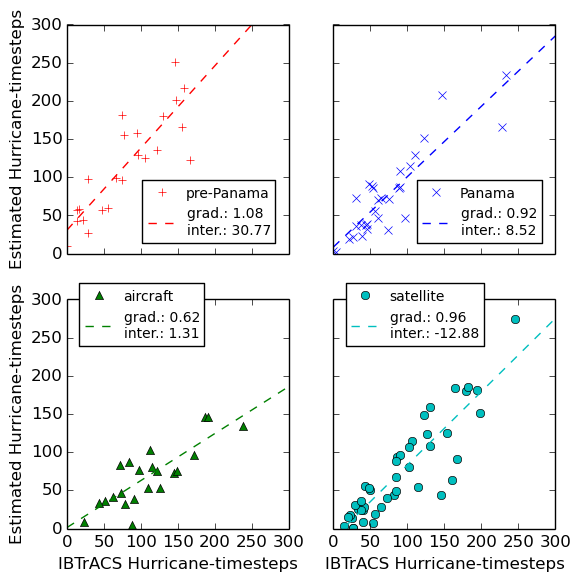
\includegraphics[width=\textwidth]{figures/20th_century_corr_split}
    \caption{Individual correlation plots for each of the four eras. $r^2$ values were between 0.68
    and 0.80, representing good correlation between the two time series for each era. The high
    gradient for the pre-Panama Canal era and the low gradient for the aircraft era are particularly
    noteworthy. }
    \label{fig:20th_century_hurricane_corr_split}
\end{figure}

\newpage
\section{Trends in Hurricane Frequencies}
\label{sec:trends_freq}

For the four eras in question, it is interesting to note whether there are any trends in the numbers
of hurricanes, both in the best tracks dataset, and in the estimated numbers. This is done by
fitting a straight line to the time series, and performing a two-sided test on the $p$ value of the
fitted line, as in \textcite{vecchi2008estimates, emanuel2010tropical}. The $p$ values for the
different eras are shown in Table \ref{tab:era_p_value}.

\begin{table}[ht!]
    \centering
    \begin{tabular}{ l | r r | r r | }
        \cline{2-5}
        & \multicolumn{2}{c |}{Best Tracks }& \multicolumn{2}{c |}{Estimated} \\
        \hline
        \multicolumn{1}{| l |}{Era} & gradient & $p$ value & gradient & $p$ value \\
        \hline
        \multicolumn{1}{| l |}{pre-Panama Canal} & -4.93 & 0.018 & -5.41 & 0.013 \\
        \multicolumn{1}{| l |}{Panama Canal} & 0.41 & 0.768 & -0.81 & 0.513 \\
        \multicolumn{1}{| l |}{Aircraft} & 1.82 & 0.391 & 0.41 & 0.768 \\
        \multicolumn{1}{| l |}{Satellite} & 1.07 & 0.190 & 2.48 & 0.001 \\
        \hline
    \end{tabular}
    \caption{Values of gradient and $p$ value of the linear regression for the best tracks and
    estimated hurricane-timestep and hurricane-timestep time series, for each of the four eras.}
    \label{tab:era_p_value}
\end{table}

\newpage
The statistical significance level is chosen to be $p = 0.05$.
This test is used to see whether the null hypothesis that the time series in question is not
changing (i.e. its gradient is zero) can be rejected. This is the same as was used in
\textcite{vecchi2008estimates}. Based on this test for significance, three of the time series over
the eras in Table \ref{tab:era_p_value} show statistically significant trends. The pre-Panama
Canal era for hurricane frequencies for best track and estimated track numbers both
show significant downwards trends. However, the most significant change is shown by the estimated
hurricane numbers in the satellite era from only the 20CR dataset, which has a $p$
value of \SI{0.001}{}, and a positive gradient. Taken at face value this implies that there is
a statistically significant positive trend over the final part of the 20\ts{th} century and start of
the 21\ts{st} century in the number of estimated hurricane-timesteps, or a rise in the frequency of hurricanes
since 1966. However, caution must be applied as there is also evidence that the number of estimated
hurricane-timesteps was below what would be expected (see Figure
\ref{fig:20th_century_hurricane_timesteps}), and therefore this rise could be due to underestimating
how many hurricanes there were in the early satellite era, rather than a genuine signal. The same
era in the best tracks number is not seen to show any significant rise, although the gradient of the
line is positive. 

% \section{Hurricane Dissipated Power Index Over the 20\ts{th} century}

\chapter{Discussion}
\label{chap:discussion}

\section{Hurricane Detection}

\subsection{Classification Success}
\label{sec:classification_success}
% Compare numbers of FP/FN/TP/TN results with walsh1997objective
% Talk about other fields that could have been collected (and the technical difficulties involved in
% doing this).  Hart parameters, temperature anomalies (go through literature and check what else is
% used and add these in). 
In one of the studies that influenced this one, \textcite{walsh1997objective} attempted to detect
cyclones in the output in T106 resolution reanalysis output. In that study, a metric called
Probability Of Detection (POD) is defined, and its definition is identical to the sensitivity used
in this study (given that missing hurricanes are added to the FN numbers, as mentioned in Section
\ref{sec:cla_successes_and_errors}). They find values of POD equal to \SI{0.57}{}, which is
lower (and therefore not as good) than the minimum values of sensitivity listed in Table
\ref{tab:classifier_performance_metrics} of \SI{0.618}{}. It is substantially lower than both the
training and validation values for the SGD classifier that was chosen in this study, which were
\SI{0.64}{} and \SI{0.68}{}. This is in spite of the fact that the resolution of the data used in
that study was almost twice as fine as the resolution used in this.

It is possibly to calculate values of PPV from the data in figures in \textcite{walsh1997objective},
although this is not done explicitly in that study. The highest value obtained is \SI{0.57}{}, which
is again lower than the values of \SI{0.74}{} (training) and \SI{0.72}{} (validation) seen in this
study for the SGD classifier. It should be pointed out that only two months, September 1989 and
October 1992, were analysed for one ensemble member there, compared with two decades with 56
ensemble members here. Therefore, due to the larger sample size, the reliability of the values in
this study should be subject to less uncertainty.

These two comparisons demonstrate the power of being able to perform classification after having
collected all the data, as well as the suitability of supervised machine learning techniques for
this task. However, sensitivities of around \SI{0.66}{} and PPVs of around \SI{0.73}{} could still
be improved upon significantly, as this represents only 66\% of actual hurricanes that are correctly
identified, and 73\% of predicted hurricanes that turn out to be actual hurricanes. 

\subsection{Improving Classification}
\label{sec:improving_classification}
During the course of this study, collecting more fields was a primary way of helping to improve
these metrics, with the temperature fields having good discriminatory power between hurricanes and
non-hurricanes.  However, there were many fields that I would have liked to have collected, but
could not, due to constraints as to what is easily available to download from the 20CR portal for
each ensemble member. These include the temperatures at \SI{700}{}, \SI{500}{} and \SI{300}{hPa},
which are used to calculate the warm core criterion and temperature anomalies
\parencite{bengtsson1995hurricane, yoshimura2006influence}. I would also have liked to have
calculated the cyclone phase space parameters as described in \textcite{evans2003objective,
hart2003cyclone}, but these require the geopotential heights of \SI{900}{}, \SI{600}{} and
\SI{300}{hPa}, and these are not readily available for each ensemble member either.  Whilst it is
possible to obtain these fields, the only way to do this is to download the entire state of the
atmosphere as represented by the GCM, which would be prohibitively time consuming for this project,
although these extra fields would have probably helped the classification procedure.

% CULLED:, although the geopotential heights of \SI{1000}{}, \SI{500}{} and \SI{200}{hPa} are.

\subsection{Tracking Algorithms}
\label{sec:discussion_tracking_algs}
% Modifications that were considered: changing other configuration parameters, Kalman Filter based
% tracker. Explain how testing framework would have allowed changes to be compared automatically,
% and to judge the success of these changes. Say that using an algorithm such as Hodges' could also
% be performed, and that this may improve the tracking noticeably.
The tracking algorithm used a simple nearest neighbour search from one timestep to another to
identify tracks. It had a few modifications, as described in Section \ref{sec:tracking}, but it
lacked the sophistication of a tracking algorithm such as the one described in
\textcite{hodges1994general, hodges1999adaptive}. In Section \ref{sec:matching}, it was
shown that the nearest neighbour tracking algorithm was capable of tracking storm systems
successfully, due to the high degree of matching between the derived tracks and the best tracks, and an
optimal configuration for the tracking was chosen based on how well the derived tracks matched the
best tracks. The suitability of the nearest neighbour tracking algorithm is supported by the low
number of missed hurricanes in each year, around 4 \% over 1990 to 2009, showing that the majority
of hurricanes recorded in the best tracks were present in the derived tracks. 

However, there were some configuration parameters that were not adjusted when working out which
configuration produced optimum tracks, such as the cutoff vorticity and distance described in Section
\ref{sec:tracking}. These may have influenced how well the derived tracks matched the best tracks,
and it would have been good to investigate the effects of using different values for these
parameters. This could be done using the general framework used in this study, which makes it easy
to objectively compare the degree of matching between the derived tracks and best tracks, as
described in Section \ref{sec:matching}. It would also allow for testing other tracking
algorithms, provided they could be made to produce data in the correct format. 

A more advanced tracking algorithm would almost certainly have produced better tracks. Referring to
the flowchart in Figure \ref{fig:hurricane_detection_proc}, it is clear that the extra field
detection and the classification do not depend on how the tracks are produced. Therefore it
should be straightforward to use a more sophisticated tracking algorithm, such as the one used in
\textcite{thorncroft2001african}. Better tracks would have lead to better estimation of where the
vorticity maxima lay, and may also have meant that fewer hurricanes were missed each year. This
could have helped to improve the reported values for sensitivity and PPV, although I believe the
changes suggested in Section \ref{sec:improving_classification} for collecting more fields
would yield greater improvements.


\section{Comparison Between Best Track and Estimated Hurricane Frequencies}
\label{sec:freq_comparison}

% Compare hurricane freqs freqemanuel2010tropical. Mention best tracks correction in
% vecchi2008estimates, and explain that the numbers that I found were in line 
Overall, there was a good correlation between the best tracks and estimated hurricane-timesteps, as
indicated by the value of $r^2 = 0.63$. From Section \ref{sec:hurr_freq_in_each_era}, the two most
striking results were that there were more estimated than best tracks hurricane-timesteps in the
pre-Panama Canal era, and that there were fewer estimated than best tracks hurricane-timesteps in
the aircraft reconnaissance era. Both of these will be considered in turn.

\subsection{Hurricane Frequencies in the Pre-Panama Canal Era}
The estimated hurricane-timesteps for the pre-Panama Canal era, 1890 - 1914, is higher than the best
tracks hurricane-timesteps. This could be an indication that there were missed hurricanes in the
best tracks dataset over this era. This is interesting because it fits in with results from previous
studies, that have taken a different approach to evaluating the reliability of best tracks datasets
in the pre-satellite era. Through analysis of correlation between Sea Surface Temperatures (SSTs)
and hurricane counts over the 20\ts{th} century, \textcite{vecchi2008estimates} have argued that
there are indeed missing hurricanes in the pre-satellite era (including the pre-Panama Canal era).
Indeed, they suggest in their study that an adjustment should be applied to hurricane frequencies in
the HURDAT database before 1966 (HURDAT is the primary source of information for storms in the North
Atlantic for IBTrACS, see Section \ref{sec:ibtracs}). This adjustment changes for each year, but for
the period from 1890 to 1914 it varies between 2.3 and 0.4 ``missing'' storms per year. This figure
is not directly comparable with the values in this study, due to a different methodology on counting
hurricanes - hurricane-timesteps were used in this study, whereas total storms were used for the
adjustment in \textcite{vecchi2008estimates}. It does however indicate that the discrepancy found in
this study could well be genuine, and offers another way of estimating how many hurricanes were
missed in the pre-satellite era.

Other studies have reach broadly the same conclusion. \textcite{landsea2007counting} finds that the
number of hurricanes was underestimated in best tracks in the early 20\ts{th} century through
comparison of hurricanes that made landfall to recorded hurricanes. \textcite{mann2007evidence} find
evidence for a ``modest undercount bias'', through use of a statistical model that links Atlantic
hurricane counts to climatic state variables. \textcite{chang2007number} reach a similar conclusion
through a consideration of hurricanes that made landfall, or got sufficiently close to land to be
detected. They find that 2.1 hurricanes per year may have been missed over the period 1904 to 1913.

\subsection{Hurricane Frequencies in the Aircraft Reconnaissance Era}
Section \ref{sec:hurr_freq_in_each_era} indicates that a number of hurricanes were missed in the
estimated hurricane-timesteps counts over the aircraft reconnaissance era. This cannot be explained
by examining the literature on missing hurricanes, as none of these studies claim that hurricanes
have been overcounted from 1944 to 1965. Although the results were not presented above, different
classifiers were run over the course of the 20\ts{th} century, and the results were broadly similar
to the results presented, in that there were fewer estimated hurricane-timesteps in the aircraft
reconnaissance era than best tracks hurricane-timesteps. This points to something going awry in the
tracking procedure, or perhaps a large number of weak hurricanes that were long in duration over
this era. This would have had the effect of the classifier classifying them as not being hurricanes,
even though they were, thus skewing the estimated hurricane-timestep numbers downwards. 

This is certainly an area which deserved more investigation and research, as it has implications
for the trends discussed in the next section, as well as casting doubts on the missing hurricanes
discussed in the previous section. This research could involve the use of different tracking
algorithms, as discussed in Section \ref{sec:discussion_tracking_algs}.

\section{Trends in Hurricane Frequencies}
% Point out numerous problems with trend analysis in hurricane frequency counts. Explain that trend
% found is probably spurious. Links to climate change and how it is quite interesting.
Two statistically significant trends were identified in Section \ref{sec:trends_freq}. The first was
found in both the best tracks and estimated hurricane-timesteps, and the second in just the
estimated hurricane-timesteps. Both will be considered in this section.

\subsection{Downward Trend in the Pre-Panama Canal Era}
The downward trends of -4.93 (best track) and -5.41 (estimated) hurricane-timesteps per year was
found to be statistically significant in both cases. This represents a downward trend from 1890 to
1914. Few studies have looked at this exact time span, so direct comparisons with the literature are
difficult. However, \textcite{vecchi2008estimates} look at the period from 1878 to 2006, and mention
two important details about the pre-Panama Canal era. The first is that there were ``high values''
in the late 1800s, which they caution could be due to greater uncertainties in the best tracks
record. The second is that there was a minimum from 1910 - 1930. Both these taken together would
mean that looking at the 1890 to 1914 period is likely to sea a downward trend, as there is a period
of high values at the start, and a period of low values at the end. That these downwards trends were
seen in both the best track and estimated hurricane-timesteps indicates that the signal is real,
although this could be a consequence of the two datasets not being fully independent, as detailed in
Section \ref{sec:ispd}.

\subsection{Upward Trend in the Satellite Era}

The fact that no statistically significant rise was found in the best tracks frequencies is of
interest, as other studies have found a rise over similar periods \parencite{goldenberg2001recent,
holland2007heightened}. However, although they both use best tracks information to draw their
conclusions, their methodology is substantially different to this study:
\textcite{goldenberg2001recent} look at ``major hurricanes'', or hurricanes that are category 3 and
above on the Saffir-Simpson scale; \textcite{holland2007heightened} use a moving average technique
for identifying trends, not the linear regression used in this study.
\textcite{vecchi2008estimates} also find a significant increase over the course of the 20\ts{th}
century, but due to differences in the time periods it is again difficult to perform a direct
comparison.

The statistically significant rise in the estimated hurricane frequencies is a significant finding.
Rises in the number of hurricanes has major socio-economic impacts, and is of contemporary interest
due to the role that climate change and global warming (particularly SST warming) has in hurricane
frequencies. However, as was mentioned before, the lower than expected counts in the early years of
the satellite era could be the reason behind this trend.

\chapter{Conclusions}
\label{chap:conclusion}
% Concluding remarks, state what I have achieved, and point out the main take home results of the
% study. Talk about how the tracking framework allows for objective comparison of different
% trackers. Talk about supervised machine learning with respect to hurricane detection, and some of the
% benefits it brings. Show that the framework of success and error metrics provides an objective way
% of measuring performance of various classifiers/detection procedures. Explain that different
% classifiers have different strengths and weaknesses, and that these can be picked in accordance
% with what is required.

% Not included in word count.
\addcontentsline{toc}{chapter}{Auto-critique}
\chapter*{Auto-critique}

% Harvard style bibliography.
\addcontentsline{toc}{chapter}{References}
\printbibliography[title={References}]

%\appendix
%\section{Additional information}

\end{document}
